\documentclass{beamer}[10]
\usepackage[portuguese]{babel}
\usepackage{pgf}
\usepackage[utf8]{inputenc}
\usepackage{beamerthemesplit}
\usepackage{graphics,epsfig, subfigure}
\usepackage{url}
\usepackage{srcltx}
\usepackage{hyperref}
\usepackage{ragged2e}
\usepackage{cancel} % para poder colocar o tracinho de cancelamento

\graphicspath{{./images/}} % set an default images folder

\definecolor{kugreen}{RGB}{50,93,61}
\definecolor{kugreenlys}{RGB}{132,158,139}
\definecolor{kugreenlyslys}{RGB}{173,190,177}
\definecolor{kugreenlyslyslys}{RGB}{214,223,216}
\setbeamercovered{transparent}
\mode<presentation>
\usetheme[numbers,totalnumber,compress,sidebarshades]{PaloAlto}
\setbeamertemplate{footline}[frame number]
\justifying

  \usecolortheme[named=kugreen]{structure}
  \useinnertheme{circles}
  \usefonttheme[onlymath]{serif}
  \setbeamercovered{transparent}
  \setbeamertemplate{blocks}[rounded][shadow=true]

\logo{
\includegraphics[width=1.55cm]{img00_UEA.png}}
%\useoutertheme{infolines} 

\title[Micro II]{Microeconomia II - 2021/02}
\author{Bruno de M. Ruas} 
\institute{Escola Superior de Ciências Sociais\\Universidade do Estado do Amazonas}
\date{\today}

\begin{document}

% pagina de titulo
\frame{\titlepage \vspace{-0.5cm}} 

% Sumario
\frame{
\frametitle{Sumário}
\tableofcontents
}

%%%%%%%%%%%%%%%%%%%%%%%%%%%%%%%%%%%%%%%%%%%
\section{Introdução}
%%%%%%%%%%%%%%%%%%%%%%%%%%%%%%%%%%%%%%%%%%%

\begin{frame}
	\Huge Introdução
\end{frame}

\begin{frame}
	\frametitle{Apresentação do Professor}
	Nome: Bruno de Melo Ruas
	\\~\\
	Formação:
	\begin{itemize}
		\item Graduação em Ciências Econômicas (UEA) em 2017
		\item Pós-graduação em Gestão Financeira (FGV) em 2020
		\item Cursando Análise e Desenvolvimento de Sistemas (PUC-MG)
	\end{itemize}

	Experiência:
	\begin{itemize}
		\item Monitorias de Intro. Eco, Macro I e Econometria
		\item Projeto Acadêmico de Iniciação Científica
		\item Observatório do Polo Industrial (UEA)
		\item Gerente de Orçamento da SEMSA-Manaus (2019-2020)
		\item Supervisor de Faturamento One Clinic (Atualmente)
	\end{itemize}
\end{frame}

\begin{frame}
	\frametitle{Ementa do Curso}
	\begin{itemize}
		\item Poder de Mercado;
		\item Monopólios e Monopsônios;
		\item Mercado de Fatores;
		\item Interação estratégica;
		\item Oligopólios: Equilíbrios de Cournot e Bertrand;
		\item Introdução à Teoria dos Jogos: Estratégias dominantes, Equilíbrio de Nash;
		\item Jogos dinâmicos, Jogos sequenciais;
		\item Introdução ao equilíbrio geral;
		\item Falhas de Mercados e ineficiência do equilíbrio;
		\item Externalidades;
		\item Bens Públicos;
		\item Assimetria de Informação.
	\end{itemize}
\end{frame}

\begin{frame}
	\frametitle{Bibliografia}
	\begin{itemize}
		\item Varian, Hal. Microeconomia: Uma Abordagem Moderna. 6 ed. Rio de Janeiro: Campus Elsevier, 2003. (Principal)
		\item Goolsbee, Levitt e Syverson. Microeconomia. 2 ed. São Paulo: Atlas, 2008.
		\item Pindyck, Robert S.; Rubinfeld, Daniel L. Microeconomia. 6 ed. São Paulo: Pearson Prentice Hall, 2007.
		\item Bergstrom, Theodore C.; Varian, Hal R. Workouts in intermediate microeconomics. WW Norton, 2014.
		\item Varian, Hal R. Intermediate microeconomics with calculus: a modern approach. WW Norton \& Company, 2014.
	\end{itemize}
\end{frame}

\begin{frame}
	\frametitle{Metodologia}
	
	Professor:
	\begin{itemize}
		\item Aulas expositivas e dinâmicas (EAD ou presenciais) com os conteúdos propostos
		\item Material didático original elaborado específicamente para o curso (versão 1.0)
		\item Grupo no discord para tiragem de dúvidas e auxílios extra-classe
		\item Publicação de todo o material no repositório do Github
	\end{itemize}

	Alunos:
	\begin{itemize}
		\item Presença participativa em todas as aulas e, em caso de falta, esforço de recuperação do material perdido
		\item Leitura antecipada do material referente à cada aula prevista
		\item Realização dos exercícios propostos em sala de aula e para casa
	\end{itemize}

\end{frame}

\begin{frame}
	\frametitle{Panorama do Curso}

	Como o nome da disciplina deixa evidente, nós estamos continuando uma jornada que já se iniciou com a disciplina de Microeconomia I.
	\\~\\
	A essa altura, você deve ter o domínio de assuntos como:
	\begin{itemize}
		\item O Modelo de Escolha do Consumidor
		\begin{itemize}
			\item Restrição Orçamentária
			\item Curvas de Indiferença
			\item Excedente do Consumidor
		\end{itemize}
		\item A Oferta da Empresa competitiva
		\begin{itemize}
			\item Custos: Médio, Marginal, Total
			\item Curvas de isolucro
			\item Tecnologias de Produção 
		\end{itemize}
		\item Mercado de Fatores
		\item O Equilíbrio de Mercado competitivo
	\end{itemize}
\end{frame}

\begin{frame}
	\frametitle{Panorama do Curso}
	Os ferramentais usados ao longo do curso de microeconomia I também não devem ser nenhum mistério. Portanto, vocês já devem saber o que são:
	\\~\\
	\begin{itemize}
		\item Funções, funções Inversas, funções lineares, coeficientes angular e linear
		\item Variações e Taxas de Variação
		\item Derivadas e Derivadas Parciais
		\item Otimização e Otimização com Restrição
	\end{itemize}
	Então podemos seguir de onde micro I parou, né?
\end{frame}

\begin{frame}
	\frametitle{Panorama do Curso}
	\begin{center}
		
\includegraphics[scale=0.4]{img01.jpg}
	\end{center}
\end{frame}

%%%%%%%%%%%%%%%%%%%%%%%%%%%%%%%%%%%%%%%%%%%
\section{Preparativos}
%%%%%%%%%%%%%%%%%%%%%%%%%%%%%%%%%%%%%%%%%%%

\begin{frame}
	\Huge Preparativos
\end{frame}

\begin{frame}
	\frametitle{Funções}
	Vamos relembrar as principais ferramentas  matemáticas necessárias para compreender alguns livros de microeconomia de graduação.
	\begin{block}{Funções}
		Sejam dois números quaisquer $x$ e $y$, uma \textbf{função} ou \textbf{transformação} é uma regra que descreve uma relação entre eles.
	\end{block}

	\begin{block}{Propriedades das Funções}
		Uma \textbf{função contínua} é aquela que não possui nenhum "salto"\ ou "quebra".\\
		Uma \textbf{função suave} é aquela que não tem "dobras"\ nem "cantos".\\
		Uma \textbf{função monotônica} é aquela que sempre segue o mesmo sentido (ou crescendo ou decrescendo) sem nunca mudar de sentido.
	\end{block}
\end{frame}

\begin{frame}
	\frametitle{Funções}

	Essas definições são simplificações draconianas dos conceitos que os matemáticos desenvolveram. Como o escopo do curso é introdutório, precisaremos nos valer dessas versões mais simples.
	\\~\\
	Quando é uma função é crescente a medida que $x$ cresce, chamaremos de \textbf{função monotônica crescente}. Quando decrescer a medida que $x$ crescer, chamaremos de \textbf{função monotônica decrescente}.

	\begin{block}{Função Inversa}
		Uma \textbf{função inversa} é a função que, sempre que colocarmos um $y$ como variável independente teremos como resultado um $x$ de alguma função anterior.
	\end{block}
\end{frame}

\begin{frame}
	\frametitle{Funções}

	\begin{block}{Função Linear}
		Chamamos de \textbf{função linear}, qualquer função da forma $y = ax + b$.
	\end{block}
	Fique atento porque uma função linear pode ser expressa de maneira implícita (ou seja, será necessário desenvolver um pouco a álgebra até que se chegue numa equação no formato da definição).
\end{frame}

\begin{frame}
	\frametitle{Equações e Identidades}
		
	\begin{block}{Equações}
		\textbf{equações} (usando o símbolo da igualdade "$=$"). Onde as suas respectivas \textbf{soluções} são os valores atribuíveis as incógnitas que assegurem a validade da relação proposta.
	\end{block}

	\begin{block}{Identidades}
		Uma \textbf{identidade} (que tem o símbolo dado por "$\equiv$") é um tipo de relação onde sempre haverá as soluções independentemente de quais valores suas variáveis assumam.
	\end{block}
\end{frame}

\begin{frame}
	\frametitle{Variações}

	\begin{block}{Variações}
		Usamos o símbolo "$\Delta$"\footnote{O nome é "delta".} para denotar a variação de alguma variável. Ou seja, se tivemos uma variável qualquer $x$ que teve seu valor alterado de $x^1$ para $x^2$, então:
		$$ \Delta x = x^2 - x^1 $$
		ou também
		$$ x^2 = x^1 + \Delta x $$
	\end{block}

	Normalmente, usamos o delta quando falamos de \textbf{pequenas variações} ou, como os economistas falam, \textbf{variações marginais}.
\end{frame}

\begin{frame}
	\frametitle{Taxa de Variação}

	\begin{block}{Taxa de Variação}
		A \textbf{taxa de variação} é obtida pela razão (ou seja, pela divisão) de duas variações. Seja a função $y = f(x)$, sempre que tivermos um $\Delta x > 0$ e também tivermos algum $\Delta y \neq 0$. A taxa de variação de $y$ em relação à $x$ é dada por:
		$$ \frac{\Delta y}{\Delta x} = \frac{y^2 - y^1}{x^2 - x^1} = \frac{f(x^1 + \Delta x) - f(x^1)}{\Delta x} $$
	\end{block}

	É uma medida do quanto $y$ varia a medida que $x$ varia.
\end{frame}

\begin{frame}
	\frametitle{Taxa de Variação}
	Quando uma função é linear, teremos que essa taxa de variação será sempre constante para quaisquer valores de $x$. Como $y = ax + b$, então
	\\~\\
	\Large $ \frac{\Delta y}{\Delta x} = $ \small
	$$ \frac{a(x^1 + \Delta x) + b - (ax^1 + b)}{\Delta x} = $$
	$$ \frac{ax^1 + a\Delta x + b - ax^1 - b}{\Delta x} = $$
	$$ \frac{ax^1 + a\Delta x \cancel{+ b} - ax^1 \cancel{- b}}{\Delta x} = $$
	$$ \frac{ax^1 + a\Delta x - ax^1}{\Delta x} = $$
	$$ \frac{\cancel{ax^1} + a\Delta x \cancel{- ax^1}}{\Delta x} = \frac{a \cancel{\Delta x}}{\cancel{\Delta x}} = a $$
\end{frame}

\begin{frame}
	\frametitle{Taxa de Variação}

	Para as funções não lineares, essa propriedade não é observada. Tomemos $y = f(x) = x^2$ como exemplo,
	\\~\\
	\Large $ \frac{\Delta y}{\Delta x} = $ \normalsize
	$$ \frac{(x + \Delta x)^2 - x^2}{\Delta x} = $$ 
	$$  \frac{\cancel{x^2} + 2x \Delta x + (\Delta x)^2 \cancel{-x^2}}{\Delta x} = $$
	$$  \frac{2x \cancel{\Delta x} + \Delta x . \cancel{\Delta x}}{\cancel{\Delta x}} = $$
	$$  2x + \Delta x $$
\end{frame}

\begin{frame}
	\frametitle{Inclinações e Interceptos}
	
	\begin{block}{Inclinações}
		Em uma função linear, a inclinação da curva sempre será a mesma independente da magnitude da variação.\\
		No caso das funções não lineares, a inclinação é dada pela \textbf{reta tangente} ao ponto da curva.
	\end{block}

	\begin{block}{Interceptos}
		No caso de uma função linear, $ y = ax + b$, temos alguns pontos que recebem nomes de \textbf{intercepto}. O \textbf{intercepto vertical} ($y^*$) é dado pelo ponto $y = a.0 + b = b$, ou seja, onde $x = 0$. Já o \textbf{intercepto horizontal} ($x^*$) é dado pelo ponto onde $y = ax + b = 0 $, ou seja, $ x = \frac{-b}{a}$
	\end{block}
\end{frame}

\begin{frame}
	\frametitle{Valor Absoluto e Logaritmo}

	\begin{block}{Valor Absluto}
		O \textbf{valor absoluto} de um número $x$ qualquer é definido pela função $f(x)$ do seguinte modo:

		\[ f(x) = |x| = \begin{cases} x & se \ x \geqslant \\ -x & se \ x < 0 \end{cases} \]
	\end{block}

	\begin{block}{Logaritmo Natural}
		Você já deve ter visto no ensino médio que o \textbf{logaritmo natural} ou \textbf{log} de um número é uma função escrita como $y = lnx$ ou $y = ln(x)$ e que possui as seguintes propriedades:

		\begin{itemize}
			\item Se $x,y > 0$, então, $ ln(xy) = ln(x) + ln(y) $
			\item $ ln(e) = 1 $
			\item $ ln(x^y) = y ln(x) $
		\end{itemize}
	\end{block}
\end{frame}

\begin{frame}
	\frametitle{Derivadas}

	Você deve lembrar desse conceito das aulas de matemática no primeiro período.
	\\~\\
	\begin{block}{Derivada}
		A \textbf{derivada} da função $f(x)$ será dada por:

		$$ f'(x) = \frac{df(x)}{dx} = \lim_{\Delta x \to 0} \frac{f(x + \Delta x) - f(x)}{\Delta x} $$
	\end{block}
	A gente acabou de ver um conceito muito parecido na parte de Taxa de Variação. E é isso mesmo, a derivada é o cálculo da taxa de variação à medida que aplicamos o limite tendendo a zero na variação de $(\Delta x)$.
\end{frame}

\begin{frame}
	\frametitle{Derivadas}

	\textbf{Comentário}: Essa técnica é muito importante ao longo de quase todos os tópicos desse curso. Volte nas apostilas e nas listas de derivadas caso seja necessário.
	\\~\\
	Já vimos que a deriva nos permite saber a inclinação da reta tangente da nossa função genérica $f(x)$ num determinado ponto.
	
	\begin{block}{Derivadas Segundas}
		Chamamos de \textbf{derivada segunda} de $f(x)$ a derivada da derivada dessa função.

		$$ f''(x) = \frac{d^2f(x)}{dx^2} $$
	\end{block}

	Se for positiva, a função é convexa no ponto. Se for negativa, a função é côncava no ponto. Por fim, se for igual a zero, a função será plana.
\end{frame}

\begin{frame}
	\frametitle{Regra do Produto e da Cadeia}

	Dadas duas funções $g(x)$ e $h(x)$.

	\begin{block}{Regra do Produto}
		Definindo uma nova função $f(x) = g(x) h(x)$. A derivada dessa última função é dada pela aplicação da \textbf{regra do produto}:
		$$ \frac{df(x)}{dx} = g(x)\frac{dh(x)}{dx} + h(x)\frac{dg(x)}{dx}$$
	\end{block}

	Dadas as funções $y = g(x)$ e $z = h(y)$.

	\begin{block}{Regra da Cadeia}
		A \textbf{função composta} é dada por $f(x) = h(g(x))$ cuja derivada de uma função composta é obtida pela \textbf{regra da cadeia} da seguinte forma:
		$$ \frac{df(x)}{dx} = \frac{dh(y)}{dy}\frac{dg(x)}{x}$$
	\end{block}
\end{frame}

\begin{frame}
	\frametitle{Derivadas Parciais}

	Supondo uma função composta $f(x_1,x_2)$.

	\begin{block}{Derivada Parcial}
		A \textbf{derivada parcial} de $f(x_1,x_2)$ em relação a $x_1$ é  dada por:

		$$ \frac{\partial f(x_1,x_2)}{\partial x_1} = 
		\lim_{\Delta x_1 \to 0} \frac{f(x_1+\Delta x_1,x_2) - f(x_1,x_2)}{\Delta x_1} $$
		\\
		Similarmente, a derivada parcial em relação a $x_2$ será dada por:
		\\
		$$ \frac{\partial f(x_1,x_2)}{\partial x_2} = 
		\lim_{\Delta x_2 \to 0} \frac{f(x_1,x_2+\Delta x_2) - f(x_1,x_2)}{\Delta x_2} $$
	\end{block}
\end{frame}

\begin{frame}
	\frametitle{Regra da cadeia das Derivadas Parciais}

	Seja a função composta $g(t) = f(x_1(t),x_2(t))$.

	\begin{block}{Regra da Cadeia para Funções Compostas}
		A \textbf{regra da cadeia} aplicada à essa função é dada por:
		$$ \frac{dg(t)}{dt} = 
		\frac{\partial f(x_1,x_2)}{\partial x_1}\frac{dx_1(t)}{dt} + 
		\frac{\partial f(x_1,x_2)}{\partial x_2}\frac{dx_2(t)}{dt} $$
	\end{block}

	Atente para o fato que as variáveis independentes da nossa função $g(t)$ são as funções $x_1(t)$ e $x_2(t)$ que também têm como variável independente $t$.
\end{frame}

\begin{frame}
	\frametitle{Otimização}

	Matematicamente falando, dada uma função $y = f(x)$ seu valor \textbf{máximo} será dado no ponto $x^*$ se $f(x^*) \geqslant f(x)$ para qualquer valor de $x$.
	\begin{block}{Condições de Maximização}
		Se uma função for suave, o seu valor máximo é obtido no ponto onde teremos:
		$$\textrm{Condição de 1º Ordem: } \frac{df(x^*)}{dx} = 0 $$
		e também
		$$\textrm{Condição de 2º Ordem: } \frac{d^2f(x^*)}{dx^2} \leq 0$$	
	\end{block}
\end{frame}

\begin{frame}
	\frametitle{Otimização}

	Também é muito comum buscarmos a minimização de determinadas funções. Nesse caso, só teremos uma pequena mudança na condição de segunda ordem

	\begin{block}{Condições de Minimização}
		Se uma função for suave, o seu valor mínimo é obtido no ponto onde teremos:
		$$\textrm{Condição de 1º Ordem: } \frac{df(x^*)}{dx} = 0 $$
		e também
		$$\textrm{Condição de 2º Ordem: } \frac{d^2f(x^*)}{dx^2} \geq 0$$	
	\end{block}
\end{frame}

\begin{frame}
	\frametitle{Otimização}

	No casos das funções compostas suaves, as condições de primeira ordem para os pontos de máximo e mínimo são alcançadas no ponto $(x_{1}^*,x_{2}^*)$ cujas derivadas serão

	\begin{block}{Otimização de Função Composta}
		$$ \frac{\partial f(x_{1}^*,x_{2}^*)}{\partial x_1} = 0 $$
		e
		$$ \frac{\partial f(x_{1}^*,x_{2}^*)}{\partial x_2} = 0 $$
	\end{block}

	As condições de segunda ordem são muito mais complexas então não fazem parte do escopo desse curso.
\end{frame}

\begin{frame}
	\frametitle{Otimização com Restrição}

	Saber maximizar ou minimizar uma função é só uma parte do problema de otimização. Na vida real, a esmagadora maioria das situações de otimização está contida dentro de algum limite de possibilidades.
	\\~\\
	A \textbf{otimização com restrição} é a técnica usada para encontrar o ponto de máximo ou mínimo de alguma função dentro de um determinado domínio de possibilidades.

	\begin{block}{Otimização com Restrição}
		$$ \huge \stackrel{max}{\textrm{\tiny $x_1,x_2$}} \normalsize f(x_1,x_2) $$
		\normalsize $$ \textrm{de modo que } g(x_1,x_2) = c $$
	\end{block}

	A função $f(x_1,x_2)$ é chamada de \textbf{função objeto} e a equação $g(x_1,x_2) = c$ é chamada de \textbf{restrição}.
\end{frame}

\begin{frame}
	\frametitle{Otimização com Restrição}

	Quando temos uma função de uma única variável, basta transformarmos a nossa restrição em uma igualdade, substituir uma função dentro da outra e aplicar as condições de primeira e segunda ordem.

	\begin{block}{Exemplo: O Problema da Empresa Líder (cap 28.2)}
		$$ \huge \stackrel{max}{\textrm{\tiny $y_1$}} \normalsize p(y_1 + y_2)y_1 - c_1(y_1) $$
		\normalsize $$ \textrm{de modo que } y_2 = f_2(y_1) $$
	\end{block}
\end{frame}

\begin{frame}
	\frametitle{Otimização com Restrição}

	Quanto temos uma função de múltiplas variáveis, temos que lidar com tangências em ordem mais elevadas. Quando dizemos que duas curvas são tangentes, podemos afirmar que o \textbf{vetor gradiente} dessas duas curvas são proporcionais em alguma medida.
	\\~\\
	Para não dificultar, um vetor gradiente é um vetor que contém as derivadas parciais de uma função multivariada. E, como qualquer vetor, poder ser somado para indicar uma única direção.
\end{frame}

\begin{frame}
	\frametitle{Otimização com Restrição}

	Num ponto qualquer $(x_1,x_2)$ o vetor gradiente aponta para a direção onde os valores da função $f(x_1,x_2)$ aumentam mais rapidamente.
	\\~\\
	Uma propriedade interessante dos vetores gradientes é que quando duas funções são tangentes, seus vetores gradientes são proporcionais. O multiplicador de Langrange é justamente a quantidade dessa proporção.
	\\~\\
	\begin{block}{Indicação de Material}
		Esse vídeo explica muito bem como o processo de otimização com restrição faz uso do vetor gradiente.
		\\
		\begin{center}
			\href{https://www.youtube.com/watch?v=yuqB-d5MjZA}{[Clique Aqui]} 
			e
			\href{https://www.youtube.com/watch?v=hQ4UNu1P2kw}{[Clique Aqui]}
		\end{center}
	\end{block}
\end{frame}

%%%%%%%%%%%%%%%%%%%%%%%%%%%%%%%%%%%%%%%%%%%
\section{Monopólio}
%%%%%%%%%%%%%%%%%%%%%%%%%%%%%%%%%%%%%%%%%%%

\begin{frame}
	\Huge Monopólio \normalsize
	\\~\\
	\begin{itemize}
		\item Maximização dos Lucros
		\item Curva de Demanda Linear e Monopólio
		\item Estabelecimento de Preços com Markup
		\item A Ineficiência do Monopólio
		\item O Ônus do Monopólio
		\item O Monopólio Natural
		\item O que Causa os Monopólios
	\end{itemize}
\end{frame}

%%%%%%%%%%%%%%%%%%%%%%%%%%%%%%%%%%%%%%%%%%%

\begin{frame}
	\frametitle{Introdução}

	Vamos trabalhar um caso diferente do que foi visto no curso de microeconomia I: \textbf{Como seria o caso onde só exista uma empresa controlando toda a oferta?}
	\\~\\
	Diferente dos casos anteriores, agora nós buscamos construir um modelo de tomada de decisão que leve em consideração a capacidade do monopolista de intervir diretamente no preço de modo a maximizar seus lucros totais.
	\\~\\
	Existem duas maneiras de enxergar esse problema:
	\begin{itemize}
		\item Podemos modelar como se o monopolista controlasse o preço e a demanda é quem definiria a quantidade de equilíbrio.
		\item Podemos modelar como se o monopolista definisse a quantidade e a demanda definiria o seu preço de equilíbrio.
	\end{itemize}
\end{frame}

%%%%%%%%%%%%%%%%%%%%%%%%%%%%%%%%%%%%%%%%%%%

\begin{frame}
	\frametitle{Maximização dos Lucros}

	Podemos resumir o problema do monopolista como:

	\begin{block}{O problema do Monopolista}
		\LARGE $$ \stackrel{max}{\text{\small $y$}} \ \ \stackrel{r(y) - c(y)}{\ } $$
	\end{block}

	Onde $p(y)$ é a demanda inversa para o mercado, $r(y) = yp(y)$ é a receita do monopolista e $c(y)$ é o custo de produção das $y$ unidades.
\end{frame}

\begin{frame}
	\frametitle{Maximização dos Lucros}

	A condição de otimização é evidente: A receita marginal deve ser igual ao custo marginal.
	\\~\\
	Se a receita marginal for maior, bastaria aumentar a produção para aumentar os lucros. Se fosse menor, seria necessário reduzir a quantidade produzida afim de elevar o preço a um nível satisfatório.
	\\~\\
	Algebricamente, o problema é
	$$ \textrm{RM = CMa} $$
	$$ ou $$
	$$ \frac{\Delta r}{\Delta y} = \frac{\Delta c}{\Delta y} $$
\end{frame}

\begin{frame}
	\frametitle{Maximização dos Lucros}

	O custo marginal é definido pela tecnologia de produção. A mudança em relação ao modelo competitivo acontecerá na receita marginal.
	\\~\\
	Como o monopolista tem o poder de intervir no mercado, sempre que ele decidir alterar a produção em $\Delta y$ unidades, haverá dois efeitos na receita:
	\begin{itemize}
		\item Ele terá um aumento na receita em $p\Delta y$ unidades
		\item Como o mercado terá mais bens a sua disposição, ele estará disposto a pagar um preço menor pelas novas unidades, ou seja, $y\Delta p$
	\end{itemize}

	O resultado será obtido por
	$$\Delta r = p \Delta y + y \Delta p$$
\end{frame}

\begin{frame}
	\frametitle{Maximização dos Lucros}

	\small $$\Delta r = p \Delta y + y \Delta p$$

	$$ \frac{\Delta r}{\Delta y} = 
	\frac{p \Delta y}{\Delta y} + 
	\frac{y \Delta p}{\Delta y} $$

	$$ \phantom{\frac{\Delta r}{\Delta y}} = 
	\frac{p \cancel{\Delta y}}{\cancel{\Delta y}} + 
	\frac{y \Delta p}{\Delta y} $$

	$$ \phantom{\frac{\Delta r}{\Delta y}} = p + y\frac{\Delta p}{\Delta y} $$

	$$ \phantom{\frac{\Delta r}{\Delta y}} = 
	p \left[ 1 + \underbrace{\frac{y}{p}\frac{\Delta p}{\Delta y}}_\text{1/elasticidade} \right] $$

	$$ \phantom{\frac{\Delta r}{\Delta y}} = 
	p \left[ 1 + \frac{1}{\epsilon(y)} \right] $$
\end{frame}

\begin{frame}
	\frametitle{Maximização dos Lucros}

	Como a elasticidade da demanda é negativa, podemos reescrever como

	$$ \frac{\Delta r}{\Delta y} = 
	RM(y) =
	p \left[ 1 - \frac{1}{|\epsilon(y)|} \right] $$

	Veja só como sofisticamos um pouco mais a ideia da receita marginal. Agora é uma função do preço e da elasticidade-preço da demanda.
	\\~\\
	Voltemos para a condição de maximização onde a Receita Marginal deve ser igual a o Custo Marginal.

	$$ p(y) \left[ 1 - \frac{1}{|\epsilon(y)|} \right] = CMa(y) $$
\end{frame}

\begin{frame}
	\frametitle{Maximização dos Lucros}

	Não faz sentido para ele operar nos pontos onde a demanda é inelástica porque ele poderia simplesmente reduzir a quantidade produzida (o que reduziria o custo total) com aumento de receita (porque o preço aumentaria). O ponto de máximo estará sempre na zona onde $|\epsilon| \geq 1$.
	\\~\\
	Se operar no ponto onde $\epsilon$ tende ao infinito, cairá exatamente no caso da competição perfeita. Onde a receita marginal é igual ao preço.
	\\~\\
	Agora podemos ver claramente que o nosso monopolista atuará somente nos pontos onde a demanda é elástica ($|\epsilon| > 1$).

	\begin{block}{Para discussão em aula}
		O que acontece quando $|\epsilon| = 1$?
	\end{block}
\end{frame}

%%%%%%%%%%%%%%%%%%%%%%%%%%%%%%%%%%%%%%%%%%%

\begin{frame}
	\frametitle{Curva de Demanda Linear e Monopólio}
	Veremos como fica o comportamento dessas variáveis num exemplo cuja curva de demanda é linear.
	\\~\\
	Considere os seguintes sistemas de equações:
	\begin{block}{Varian pg 632}
		$$ \textrm{Demanda Linear Inversa: } p(y) = a - by $$
		$$ \textrm{Função Receita: } r(y) = p(y)y = ay - by^2 $$
		$$ \textrm{Função Receita Marginal: } RM(y) = a - 2by $$
	\end{block}

	A receita marginal é dada (capítulo 15) pela derivada da função receita. Podemos ver que o intercepto vertical da demanda e da receita marginal são iguais (dado pelo ponto $a$).
\end{frame}

\begin{frame}
	\frametitle{Curva de Demanda Linear e Monopólio}

	\begin{center}
		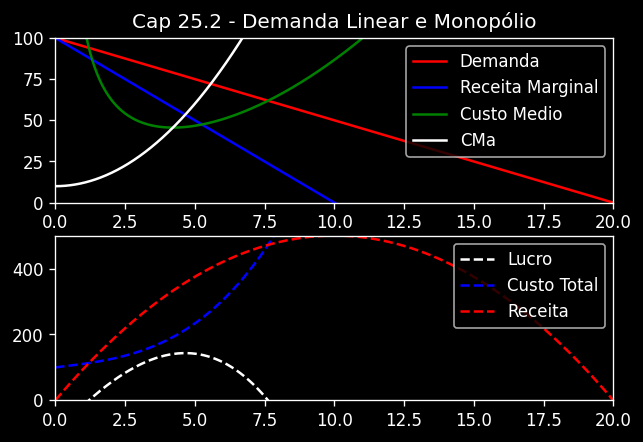
\includegraphics[scale=0.7]{cap25_2-demanda_linear_e_monopolio.png}
	\end{center}
	
\end{frame}

\begin{frame}
	\frametitle{Curva de Demanda Linear e Monopólio}

	Conseguimos ver que a curva de lucro tem um ponto de máximo exatamente onde a curva da receita marginal encontra o custo marginal. Qualquer ponto diferente desse levaria a um nível de lucro menor.
	\\~\\
	Além disso, também é relevante o fato da curva de custo médio estar abaixo da curva de demanda. Se o ponto de produção cuja receita marginal é igual ao custo marginal tiver um custo médio superior a demanda, a empresa receberá menos do que os custo de produção.
\end{frame}

%%%%%%%%%%%%%%%%%%%%%%%%%%%%%%%%%%%%%%%%%%%

\begin{frame}
	\frametitle{Estabelecimento de Preços com Markup}
	
	Agora que tornamos a receita marginal endógena, podemos ver as condições de maximização do lucro quando a firma tem poder de definir o preço ou a quantidade do mercado (mas não os dois ao mesmo tempo).
	\\~\\
	Podemos compreender essa última equação como uma política de preço do monopolista. Para isso, só precisamos isolar o termo $p(y)$ via rearranjo da última equação, o que após feito nos dá a seguinte relação

	$$ p(y) = \frac{CMa(y)}{1 - 1/|\epsilon(y)|} $$

	Essa equação nos diz que o preço praticado no mercado cujo monopolista atua sempre se comportará como uma função de \textit{markup} do seu custo marginal.
\end{frame}

\begin{frame}
	\frametitle{Estabelecimento de Preços com Markup}

	Podemos simplificar a visualização disso do seguinte modo
	
	$$ p(y) = \phi \times CMa(y) $$
	
	onde $\phi = \frac{1}{1 - 1/|\epsilon(y)|}$.
	\\~\\
	Como sabemos, o monopolista sempre operará nos pontos cuja demanda é elástica, isso nos dará um $\epsilon(y) > 1$. Isso nos diz que o divisor $(1 - 1/|\epsilon|) <  1$, o que por sua vez, nos diz que $\phi > 1$.

	\begin{block}{Para dicussão em aula - Varian pg 634}
		Vamos analisar o caso da modelagem para um mercado com demanda de elasticidade constante.
	\end{block}
\end{frame}

%%%%%%%%%%%%%%%%%%%%%%%%%%%%%%%%%%%%%%%%%%%

\begin{frame}
	\frametitle{A Ineficiência do Monopólio}
	
	Já conseguimos ver que, quando uma empresa opera como um monopólio, o preço de mercado será definido sempre acima do seu custo marginal.
	\\~\\
	No mercado de competição perfeita, esse preço seria exatamente igual ao custo marginal. 
	\\~\\
	Isso implica na redução de algum excedente dos consumidores, mas em um incremento no excedente do produtor.
	\\~\\
	Como já sabemos, um arranjo é eficiente no sentido de Pareto se, e somente se, é possível realizar alguma troca de modo a se ter um aumento no excedente de uma das partes sem a redução do excedente de outra parte.
\end{frame}

\begin{frame}
	\frametitle{A Ineficiência do Monopólio}
	
	Agora vamos investigar se o equilíbrio no mercado monopolista é eficiente. Considere a imagem abaixo.
	\begin{center}
		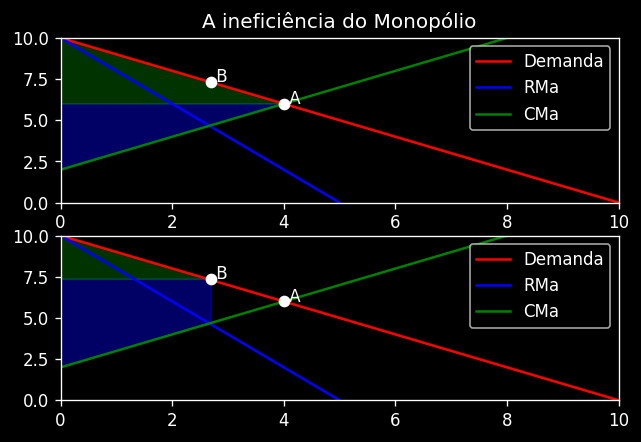
\includegraphics[scale=0.6]{cap25_4-inef_monopolio.png}
	\end{center}
\end{frame}

\begin{frame}
	\frametitle{A Ineficiência do Monopólio}
	
	O gráfico da parte de cima é o equilíbrio no mercado de competição e o de baixo é o nosso equilíbrio com monopólio.
	\\~\\
	Perceba como há um incremento no excedente do produtor (medido pela área azul) e uma redução do excedente do consumidor (área verde).
	\\~\\
	Para investigarmos se há uma ineficiência no sentido de Pareto no ponto $B$, façamos a seguinte pergunta: 
	\begin{block}{Para discussão em aula}
		É possível adicionar uma unidade de produto no mercado de modo que o custo marginal pela produção desse bem seja inferior ao preço do mesmo?
	\end{block}	
\end{frame}

\begin{frame}
	\frametitle{A Ineficiência do Monopólio}
	
	No nível $B$, a curva de preço (medida pela demanda inversa) ainda é superior à curva de custo marginal (aquela reta verde).
	\\~\\
	Desse modo, se o monopolista produzisse mais uma unidade, ele receberia mais do que o custo marginal dessa unidade e os consumidores cujo preço de reserva é igual ao novo nível de preço passariam a consumir o produto.
	\\~\\
	Como o produtor teria um lucro positivo (pois o custo marginal é inferior ao preço) e os consumidores teriam um aumento de excedente, achamos uma melhoria de Pareto.
	\\~\\
	Com isso, podemos ver que o equilíbrio com monopólio é ineficiente no sentido de Pareto.
\end{frame}

%%%%%%%%%%%%%%%%%%%%%%%%%%%%%%%%%%%%%%%%%%%

\begin{frame}
	\frametitle{O Ônus do Monopólio}
	
	Agora que já vimos que o monopólio é ineficiente, podemos querer mensurar o tamanho dessa ineficiência.
	\\~\\
	Uma maneira possível de medir essa ineficiência é observando os excedentes nos cenários competitivo e de monopólio. Observe a figura abaixo:
	
	\begin{center}
		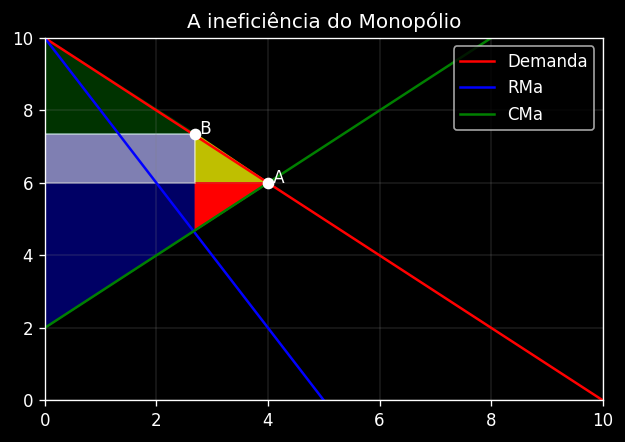
\includegraphics[scale=0.5]{cap25_5-onus_monopolio.png}
		\end{center}
\end{frame}

\begin{frame}
	\frametitle{O Ônus do Monopólio}
	
	A área amarela é a medida da redução do excedente do consumidor.
	\\~\\
	Em vermelho temos a redução do excedente do produtor.
	\\~\\
	Em branco temos o quanto o monopolista consegue "capturar"\ do excedente dos consumidores ao adotar o nível de produção que maximiza o seu lucro.
	\\~\\
	O \textbf{ônus resultante do monopólio} é precisamente a soma das áreas amarela e vermelha.
\end{frame}

%%%%%%%%%%%%%%%%%%%%%%%%%%%%%%%%%%%%%%%%%%%

\begin{frame}
	\frametitle{O Monopólio Natural}

	Já aprendemos o modelo de decisão do monopolista e também já vimos a ineficiência que esse modelo acarreta para os mercados.
	\\~\\
	Ao percebemos que o monopólio produz aquém da quantidade ótima, poderíamos nos sentir tentados a propor regulações que obrigassem o monopolista a aumentar o seu nível de produção até o nível da competição perfeita.
	\\~\\
	Contudo, esse problema é mais complexo do que parece, porque essa proposta de solução não leva em consideração a estrutura de custos.
	\\~\\
	A próxima imagem é um exemplo do que acontece quando alteramos apenas o custo fixo em 3 diferentes cenários.
\end{frame}

\begin{frame}
	\frametitle{O Monopólio Natural}
	\begin{center}
		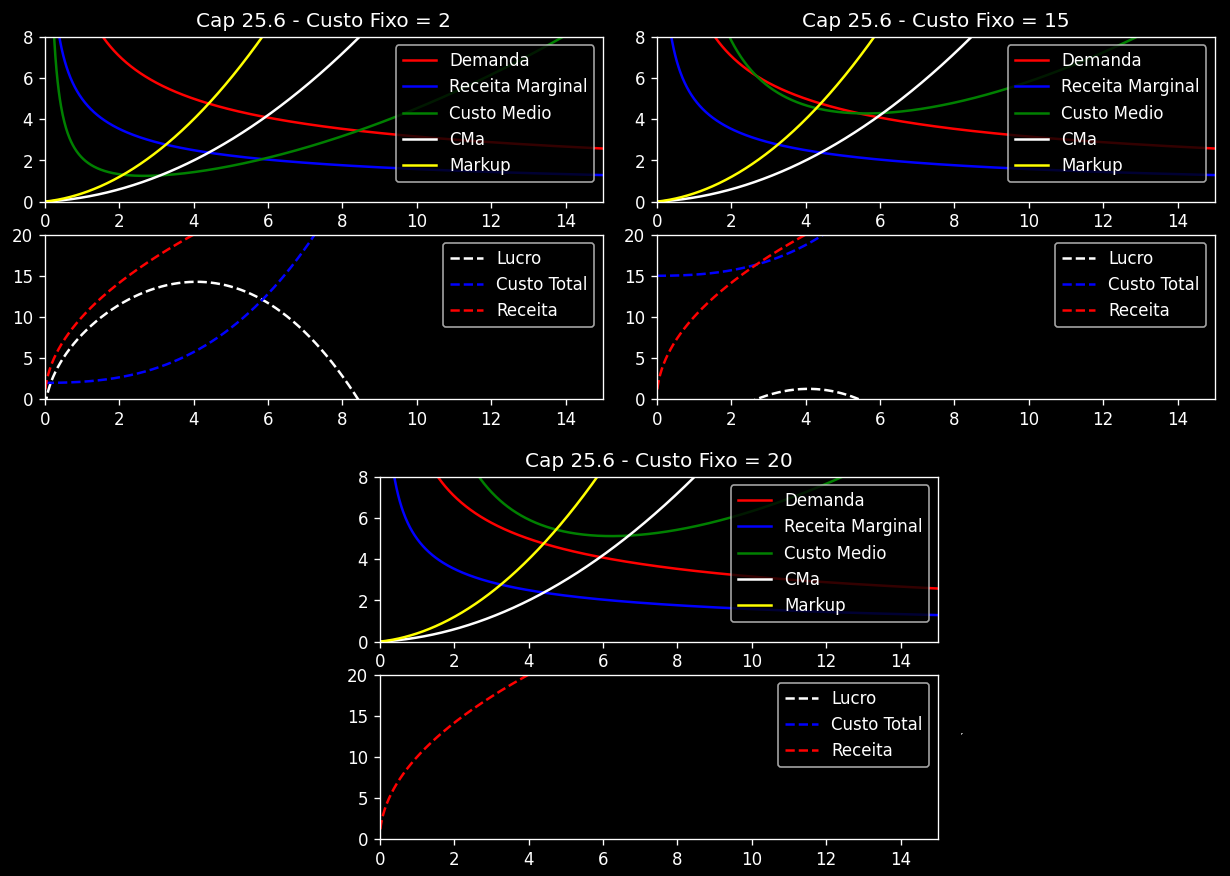
\includegraphics[scale=0.3]{cap25_6-monopolio_natural.png}
		\end{center}
\end{frame}

\begin{frame}
	\frametitle{O Monopólio Natural}

	Chamamos de \textbf{monopólio natural} a situação onde temos uma estrutura de custo fixos muito alta e custos marginais baixos.
	\\~\\
	Agora podemos ver que se obrigarmos o monopolista a produzir o nível da competição perfeita, pode acontecer do projeto não ser sustentável, pois a curva de custo médio está acima da curva de demanda.
	\\~\\
	Não existe solução simples para essa questão. Na maioria das situações os monopólios naturais são regulamentados ou operados diretamente pelos governos.
	\\~\\
	Cada opção de solução acaba acarretando benefícios e malefícios consigo. Em ambos os casos, os problemas são geralmente oriundos devido a informação assimétrica entre a empresa e os seus controladores.
\end{frame}

%%%%%%%%%%%%%%%%%%%%%%%%%%%%%%%%%%%%%%%%%%%

\begin{frame}
	\frametitle{O que Causa os Monopólios?}

	Agora nos resta uma última investigação: Qual a causa dos monopólios?
	\\~\\
	Uma variável que podemos creditar como importante é a \textbf{escala mínima de eficiêntia (EME)}. Ela nada mais é do que o ponto de mínimo da nossa curva de custo médio.
	\\~\\
	O formato da curva de custo médio (e consequentemente a EME) é definido exclusivamente pela tecnologia.
	\\~\\
	Quando temos uma escala mínima de eficiência muito elevada, uma empresa precisa produzir uma quantidade muito grande dos bens vendidos no mercado para se manter.
\end{frame}

\begin{frame}
	\frametitle{O que Causa os Monopólios?}
	Quando temos uma EME pequena, qualquer empresa pequena pode começar a operar no mercado. Isso aumenta o número de competidores.
	\\~\\
	O que acaba por reduzir o peso de cada empresa individualmente. O que acaba por gerar um ambiente de competição.
	\\~\\
	Observe que o fator importante é a relação entre a EME e o tamanho do mercado. Se a EME é de 10.000 unidades, mas o mercado é o país todo, essa é uma EME relativamente baixa. Se o tamanho do mercado fosse um único shopping center, aí seria considerar consideravelmente alta.
\end{frame}

\begin{frame}
	\frametitle{O que Causa os Monopólios?}
	Além da EME, outra maneira de se criar um monopólio é por meio da coordenação dos agentes ofertantes em uma \textbf{colusão}.
	\\~\\
	Quando um conjunto de empresa se une para definir em conjunto a produção, elas agem como um \textbf{cartel}.
	\\~\\
	Esse cartel acaba atuando como se fosse um ofertante só (e consequentemente, age com o poder de mercado advindo dessa coordenação).
\end{frame}

\begin{frame}
	\frametitle{O que Causa os Monopólios?}
	Um terceiro e último motivo para o nascimento de um monopólio é o bom e velho "cheguei primeiro".
	\\~\\
	Se uma empresa, por algum acidente histórico, é a primeira a se estabelecer no mercado. É natural que ela se valha da falta de competidores e consiga um crescimento em escala.
	\\~\\
	Quando novos ofertantes entram no mercado, o monopolista consegue usar seu arsenal de escala e reduzir artificialmente o preço até o ponto onde ninguém além dele pode se manter.
\end{frame}

%%%%%%%%%%%%%%%%%%%%%%%%%%%%%%%%%%%%%%%%%%%
\section{C. Monopólio}
%%%%%%%%%%%%%%%%%%%%%%%%%%%%%%%%%%%%%%%%%%%

\begin{frame}
	\huge O comportamento do Monopolista \normalsize
	\\~\\
	\begin{itemize}
		\item Tipos de discriminação de preços
		\item Discriminação de 1º ordem
		\item Discriminação de 2º ordem
		\item Discriminação de 3º ordem
		\item Vinculação de produtos
		\item Tarifas bipartidas
		\item Competição monopolística
		\item Estabilidade na Competição
		\item Diferenciação de Produtos
		\item Mais sorveteiros
	\end{itemize}
\end{frame}

%%%%%%%%%%%%%%%%%%%%%%%%%%%%%%%%%%%%%%%%%%%

\begin{frame}
	\frametitle{Tipos de Discriminação de Preços}

	Nós vimos que o monopolista acaba produzindo em um ponto onde a demanda ainda está disposta a pagar por mais do que o custo marginal.
	\\~\\
	Porque o monopolista não abaixa o preço para vender mais unidades?
	\\~\\
	Ele teria de baixar o preço de todos os produtos e não apenas os adicionais!
	\\~\\
	Existem alguns monopolistas que detém o poder de \textbf{discriminação de preços}.

\end{frame}

\begin{frame}
	\frametitle{Tipos de Discriminação de Preços}

	\begin{itemize}
		\item Discriminação de Preços de 1º Grau:
			\begin{itemize}
			\item[] Nesse caso ele tem poder de cobrar um preço diferente para cada consumidor e para cada quantidade.
			\end{itemize}
		\item Discriminação de Preços de 2º Grau
			\begin{itemize}
			\item[] Nesse caso ele tem poder de discriminar o preço apenas para as quantidades compradas. Mas todos os consumidores que levarem a mesma quantidade, pagarão o mesmo preço no total.
			\end{itemize}
		\item Discriminação de Preços de 3º Grau
			\begin{itemize}
			\item[] Esse é o caso mais comum. É quando o monopolista tem o poder de escolher qual preço cada pessoa vai pagar por todas as unidades que levar. Ou seja, ele pode controlar qual o valor de todas as unidades da cesta, contudo, não pode diferenciar o valor entre essas unidades.
			\end{itemize}
		\end{itemize}

\end{frame}

%%%%%%%%%%%%%%%%%%%%%%%%%%%%%%%%%%%%%%%%%%%

\begin{frame}
	\frametitle{Discriminação de Preços de 1º Grau}

	O monopolista está em plenos poderes. Ele possui conhecimento do preço de reserva de cada consumidor e, com esse conhecimento, cobra exatamente o valor máximo para cada quantidade. Também chamamos esse tipo de \textbf{discriminação perfeita}.
	\\~\\
	Um fato curioso desse arranjo é que, por incrível que pareça, ele é eficiente no sentido de Pareto.
	
	\begin{block}{Para discussão em aula}
		Quem pode explicar como esse arranjo pode ser ótimo de Pareto?
	\end{block}

	Em termos de excedente, o que acontece é que o monopolista captura todo o excedente do mercado. Os consumidores, por sua vez, não possuem nenhum excedente.
\end{frame}

\begin{frame}
	\frametitle{Discriminação de Preços de 1º Grau}

	\begin{figure}[H]
		\centering
		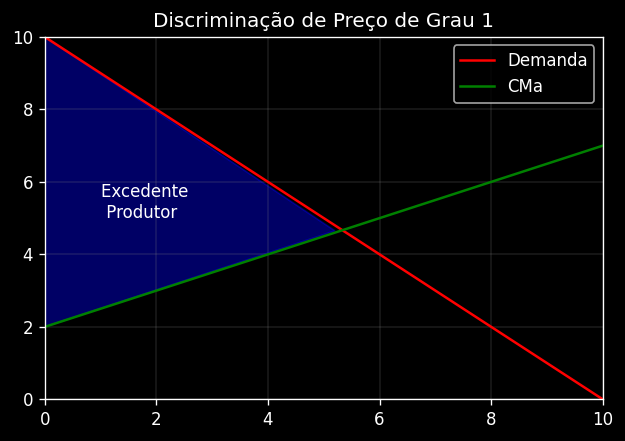
\includegraphics[scale=0.75]{cap26_2-discriminacao_grau1.png}
	\end{figure}

\end{frame}

\begin{frame}
	\frametitle{Discriminação de Preços de 1º Grau}

	Um exemplo é o mafioso Don Vito Corleone da clássica trilogia de filmes The Godfather. O "modelo de negócio"\ do protagonista é fazer alguns favores em troca de outros favores. No caso do personagem mafioso, ele abusava do poder de mercado que detinha para cobrar o máximo possível (em bens ou serviços) de quem estava em dívida com ele.

	\begin{figure}[H]
		\centering
		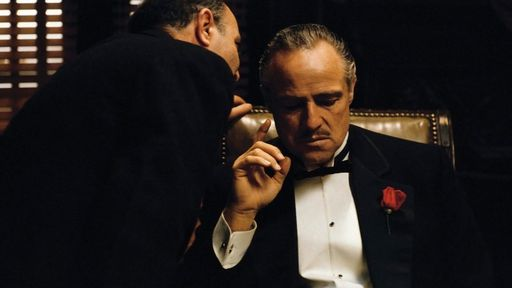
\includegraphics[scale=0.3]{cap26_2-don_corleone.jpeg}
	\end{figure}

\end{frame}

\begin{frame}
	\frametitle{Discriminação de Preços de 2º Grau}

	Nesse modelo, também chamado de \textbf{fixação de preços não linear}, o produtor já não pode cobrar, por uma mesma quantidade, um valor diferente entre consumidores diferentes.
	\\~\\
	Isso força o monopolista a desenvolver uma estratégia de precificação que tente tirar o maior proveito possível das diferentes curvas de demanda.
	\\~\\
	Imagine que temos apenas 2 grupos de consumidores no mercado. Como nosso modelo prevê, o monopolista tem acesso as curvas de demanda de cada consumidor, mas como limitação, ele só pode escolher quais cestas ofertar por qual preço, e deixar que os consumidores escolham qual é a melhor para eles.

\end{frame}

\begin{frame}
	\frametitle{Discriminação de Preços de 2º Grau}

	O objetivo do monopolista é captar todo o excedente do mercado. Mas ele enfrenta uma limitação nessa modalidade de discriminação de preços.
	\\~\\
	Como ele não pode vender a mesma quantidade a preços diferentes para os grupos de consumidores, ele tem de escolher se vai vender a preço de reserva da curva de demanda 1 ou 2.
	\\~\\
	Se ele optar por vender na fronteira da curva de demanda 1, ele vai abrir mão de todo o excedente advindo dos consumidores do tipo 2!

\end{frame}

\begin{frame}
	\frametitle{Discriminação de Preços de 2º Grau}

	\begin{figure}[H]
		\centering
		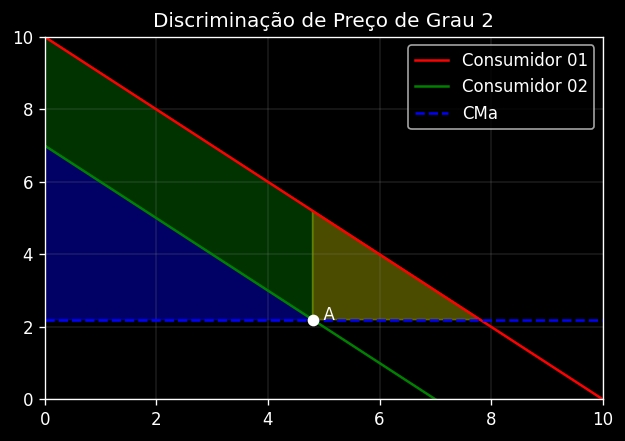
\includegraphics[scale=0.7]{cap26_3-discriminacao_grau2_1.png}
	\end{figure}
	
\end{frame}

\begin{frame}
	\frametitle{Discriminação de Preços de 2º Grau}

	\begin{figure}[H]
		\centering
		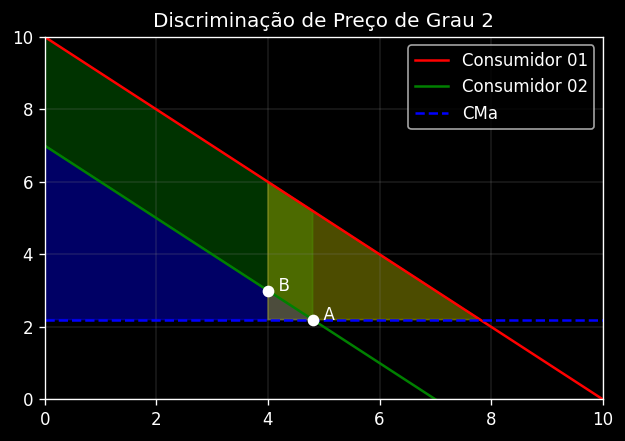
\includegraphics[scale=0.7]{cap26_3-discriminacao_grau2_2.png}
	\end{figure}
	
\end{frame}

\begin{frame}
	\frametitle{Discriminação de Preços de 2º Grau}

	\begin{figure}[H]
		\centering
		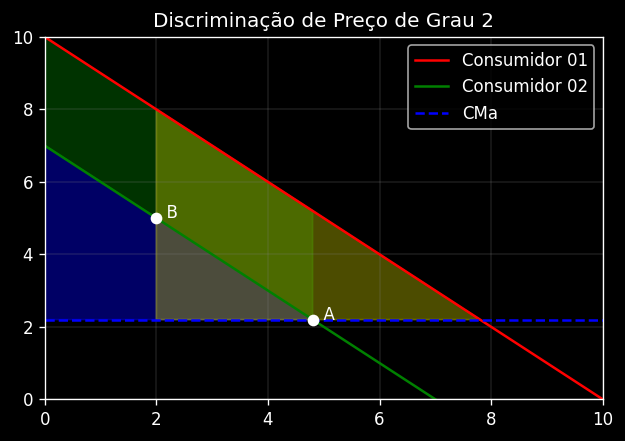
\includegraphics[scale=0.7]{cap26_3-discriminacao_grau2_3.png}
	\end{figure}
	
\end{frame}

\begin{frame}
	\frametitle{Discriminação de Preços de 2º Grau}

	Na realidade, o principal método de incentivo a autosseleção é a alteração da qualidade do bem. Normalmente, o monopolista reduz a qualidade dos produtos direcionados aos consumidores com preços de reserva menores, afim de evitar que seus consumidores dispostos a pagar mais, prefiram comprar esses produtos ao invés de produtos de "primeira linha".
	\\~\\
	Essa estratégia maximiza o lucro do monopolista e ainda garante algum excedente para os consumidores das demandas mais altas.

	\begin{figure}[H]
		\centering
		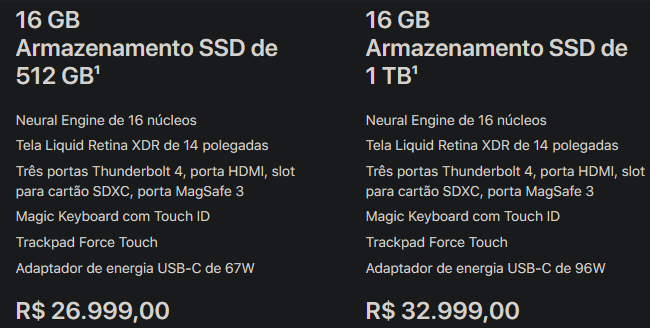
\includegraphics[scale=0.3]{cap26_3-discriminacao_grau2_4.png}
	\end{figure}

\end{frame}

%%%%%%%%%%%%%%%%%%%%%%%%%%%%%%%%%%%%%%%%%%%

\begin{frame}
	\frametitle{Discriminação de Preços de 3º Grau}

	Nesse caso, o monopolista consegue discernir claramente qual consumidor pertence a qual grupo e, consequentemente, consegue cobrar um preço diferente. Atente para o fato que o monopolista só pode adota um único preço para cada grupo de consumidores.
	\\~\\
	Na prática, a modelagem desse problema é muito parecida com o que vimos no capítulo passado, já que, ele só pode escolher um único preço para cada tipo de consumidor.
	\\~\\
	A única diferença do modelo do capítulo passado é que ele vai se deparar com mais de uma curva de demanda.

\end{frame}

\begin{frame}
	\frametitle{Discriminação de Preços de 3º Grau}

	\begin{center}
		\LARGE $\stackrel{max}{\text{\small $y_1,y_2$}} \ \  \stackrel{p_1(y_1)y_1 + p_2(y_2)y_2 - c(y_1 + y_2)}{\ }$ \\
	\end{center}

	$$ RM_1(y_1) = CMa(y_1+y_2) $$
	$$ RM_2(y_2) = CMa(y_1+y_2) $$

	\begin{center}
		Isso claramente implica em
	\end{center}

	$$ RM_1(y_1) = RM_2(y_2) = CMa(y_1+y_2) $$

\end{frame}

\begin{frame}
	\frametitle{Discriminação de Preços de 3º Grau}

	Podemos usar a nossa fórmula da elasticidade para elaborar um pouco mais esse problema:

	$$ p_1(y_1) \left[1 - \frac{1}{|\epsilon_1(y_1)|} \right] = CMa(y_1 + y_2) $$
	$$ p_2(y_2) \left[1 - \frac{1}{|\epsilon_2(y_2)|} \right] = CMa(y_1 + y_2) $$

	Suponha que $y_1 = y_2$. Se $p_1 > p_2$, então:

	$$ 1 - \frac{1}{|\epsilon_1(y_1)|} < 1 - \frac{1}{|\epsilon_2(y_2)|} $$

\end{frame}

\begin{frame}
	\frametitle{Discriminação de Preços de 3º Grau}

	O que implica em

	$$ \frac{1}{|\epsilon_1(y_1)|} > \frac{1}{|\epsilon_2(y_2)|} $$

	Que, por fim, nos diz que

	$$ |\epsilon_1(y_1)| < |\epsilon_2(y_2)| $$

\end{frame}

\begin{frame}
	\frametitle{Discriminação de Preços de 3º Grau}

	Vocês agora entendem o motivo de existir meia entrada.
	\\~\\
	Eu sei, eu sei, isso é muito top.
	\\~\\
	O monopolista vai cobrar mais caro de quem tiver a demanda menos elástica.

\end{frame}

\begin{frame}
	\frametitle{Discriminação de Preços de 3º Grau}

	\begin{figure}[H]
		\centering
		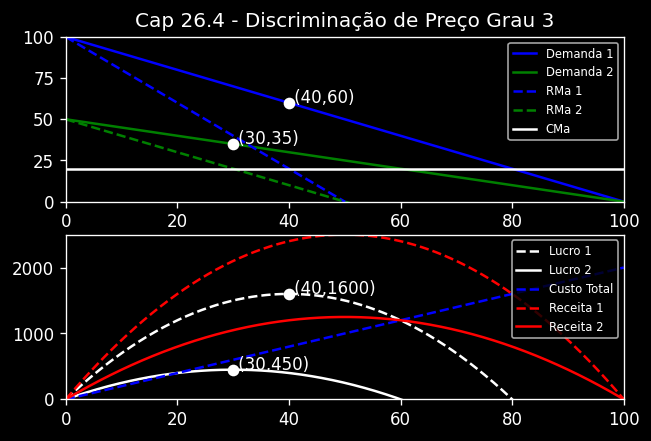
\includegraphics[scale=0.7]{cap26_4-discriminacao_grau3.png}
	\end{figure}

\end{frame}

\begin{frame}
	\frametitle{Discriminação de Preços de 3º Grau}

	\begin{figure}[H]
		\centering
		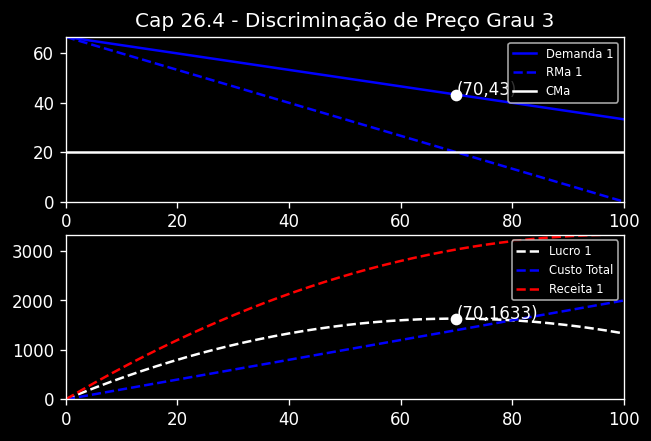
\includegraphics[scale=0.7]{cap26_4-discriminacao_grau3_2.png}
	\end{figure}

\end{frame}

%%%%%%%%%%%%%%%%%%%%%%%%%%%%%%%%%%%%%%%%%%%

\begin{frame}
	\frametitle{Vinculação de Produtos}

	Já vimos que a vontade do monopolista é cobrar o máximo possível para cada cliente em cada quantidade. Isso faria com que ele capturasse todo o excedente do mercado. 
	\\~\\
	Como na prática isso implicaria em conhecimento perfeito de todos os consumidores e existe uma legislação que limita a capacidade de impor muito do poder de mercado, as empresas se valem de estratégias para maximizar esse excedente.
	\\~\\
	Uma dessas estratégias é exatamente a venda casada. A ideia é a seguinte: como o vendedor não pode cobrar um preço para cada consumidor, ele precisa ter uma ideia dos preços de reserva dos mesmos para que possa cobrar exatamente o valor do preço de reserva mais baixo que o custo marginal permita.

\end{frame}

\begin{frame}
	\frametitle{Vinculação de Produtos}

	\begin{center}
		\begin{tabular}{ |c|c|c| } 
		 \hline
		 Consumidor & Processador Texto & Planilha Eletrônica \\ 
		 \hline
		 A & 120 & 100 \\ 
		 B & 100 & 120 \\ 
		 \hline
		\end{tabular}
	\end{center}

	\begin{block}{Para discussão em aula}
		Vale mais a pena o monopolista cobrar separadamente ou pela cesta dos dois bens?
	\end{block}

\end{frame}

%%%%%%%%%%%%%%%%%%%%%%%%%%%%%%%%%%%%%%%%%%%

\begin{frame}
	\frametitle{Tarifas Bipartidas}

	Baseado no paper de Walter Oi, "A Disneyland Dilemma: Two-Part Tariffs for a Mickey Mouse Monopoly".
	\\~\\
	Como o monopolista se comportará no caso da venda de dois produtos que possuem demandas interrelacionadas?
	\\~\\
	No tópico anterior, supomos que as demandas eram independentes. Agora temos um caso onde, ao aumentar a oferta do bem 1, os consumidores estarão menos propensos a consumir o bem 2. Chamamos esse arranjo de \textbf{tarifa bipartida}.

\end{frame}

\begin{frame}
	\frametitle{Tarifas Bipartidas}

	Como já trabalhamos antes, sabemos que a maximização do lucro é obtida no ponto onde o custo marginal é igual à receita marginal. 
	\\~\\
	Fazendo isso para a oferta do bem 1 e como ele não pode discriminar perfeitamente os preços, haverá um excedente do consumidor. Esse excedente é exatamente o valor máximo que ele pode cobrar pelo bem 2. 
	\\~\\
	Nesse caso, pode ser que a quantidade cobrada pelo bem 2 seja inferior ao montante que iguale o custo marginal à receita marginal.
\end{frame}

\begin{frame}
	\frametitle{Tarifas Bipartidas}

	\begin{figure}[H]
		\centering
		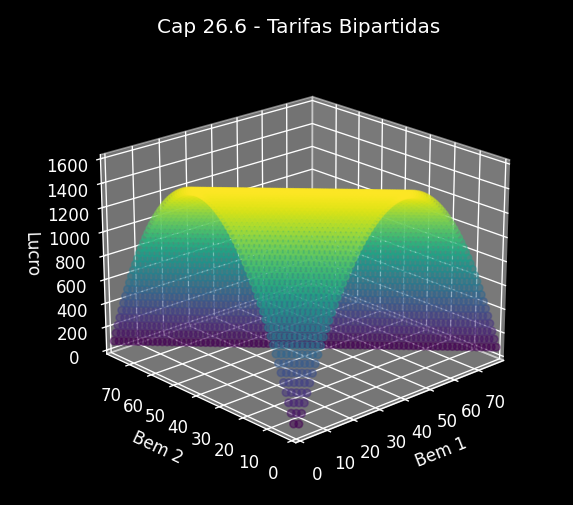
\includegraphics[scale=0.7]{cap26_6-tarifas_bipartidas3.png}
	\end{figure}

\end{frame}

%%%%%%%%%%%%%%%%%%%%%%%%%%%%%%%%%%%%%%%%%%%

\begin{frame}
	\frametitle{Competição Monopolística}

	Nós começamos essa seção do livro partindo da posição oposta aos modelos que vimos ao longo da primeira metade do curso.
	\\~\\
	Adaptamos o modelo da escolha maximizadora do lucro para a existência do poder de mercado e avançamos como o monopolista pode usar esse poder mesmo em arranjos menos favoráveis à capacidade de discriminação de preços.
	\\~\\
	Nessas últimas duas seções expandimos nosso modelo para mais de um produto e como eles podem interagir entre si para a maximização do lucro.

\end{frame}

\begin{frame}
	\frametitle{Competição Monopolística}

	Até agora, tratamos uma \textbf{indústria} como um conjunto de produtores cujo resultado do esforço produtivo era \textit{exatamente} a mesma mercadoria. Isso quer dizer que, sendo 1 (que é o caso do monopólio) ou 1.000 produtores, todas as mercadorias que saem das fábricas e são comercializadas seriam exatamente as mesmas. 
	\\~\\
	Essa hipótese simplificadora vai dar lugar a uma nova que, na minha opinião, é bem mais aplicável a nossa realidade fática.
	\\~\\
	Os produtos agora possuem certas propriedades exclusivas (sendo a marca a principal) e seus competidores também serão diferenciáveis entre si. Todos competindo por um mercado de bens relativamente parecidos aos consumidores.

\end{frame}

\begin{frame}
	\frametitle{Competição Monopolística}

	Nesse novo arranjo, os produtores possuem características de ambos os modelos vistos. 
	\\~\\
	Eles não podem alterar seus preços completamente como um monopólio, porque os consumidores olhariam para os seus concorrentes e comprariam algum produto semelhante ao seu, só que mais barato. 
	\\~\\
	Por outro lado, eles não estão fadados estritamente ao preço de mercado, uma vez que nesse arranjo a demanda não será infinitamente elástica. 
	\\~\\
	O nome dessa estrutura setorial é \textbf{concorrência monopolística}.

\end{frame}

\begin{frame}
	\frametitle{Competição Monopolística}

	É razoável supor que se o número de concorrentes aumentar (algo que está muito relacionado às barreiras de entrada) haverá impactos na curva de demanda que a empresa está imposta.
	\\~\\
	O primeiro impacto que podemos supor é que essa curva irá se aproximar mais da origem do plano cartesiano. Ou seja, ele vai acabar tendo que baixar mais o seu preço se quiser continuar vendendo a mesma quantidade.
	\\~\\
	O segundo impacto previsto é que a elasticidade de demanda aumentará porque agora os consumidores podem escolher mais opções em relação a antes.

\end{frame}

\begin{frame}
	\frametitle{Competição Monopolística}

	Se todas as empresas do mercado tiverem como objetivo o lucro. Qualquer equilíbrio alcançado terá que obedecer algumas restrições:

	\begin{itemize}
		\item Cada empresa venderá o máximo possível. Ou seja, elas sempre optam por ofertar cestas que estejam na curva de demanda e não abaixo dela.
		\item Cada empresa precisará maximizar seu lucro levando em consideração as imposições oriundas à sua curva de demanda da empresa.
		\item Quanto mais competidores o mercado tiver, mais próximo de zero será o lucro das empresas contidas no mercado.
	\end{itemize}

\end{frame}

\begin{frame}
	\frametitle{Competição Monopolística}

	Do fato 1, podemos derivar o fato que quaisquer opções de maximização estão na própria curva de demanda.
	\\~\\
	Do fato 3, podemos ver que a medida que o número de competidores tende ao infinito, a cesta escolhida deve ser num ponto onde a curva de custo médio tangencia a curva de demanda.
	\\~\\
	Por fim, o nosso postulado 2 afirma que a maximização ocorrerá na curva de demanda, isso implica no fato que a curva de custo médio não cruzará a curva de demanda, porque se isso acontecer, as empresas terão lucro positivos.
\end{frame}

%%%%%%%%%%%%%%%%%%%%%%%%%%%%%%%%%%%%%%%%%%%

\begin{frame}
	\frametitle{Estabilidade na Competição}

	Esse seção é inspirada no clássico artigo de 1929 "Stability in Competition"\ de Harold Hotelling. Isso mesmo, 1929.
	\\~\\
	Imagine que a orla da Ponta Negra seja retilínea e que só seja permitida a venda de sorvetes mediante autorização da Prefeitura. Adicionaremos a restrição que a probabilidade de você encontrar um transeunte com calor é uniforme em toda a extensão da orla. Suporemos também que os preços dos sorvetes sempre serão iguais, que não há diferença de qualidade e que por motivos climáticos só exista um único sabor disponível.
	\\~\\
	Diante das características do mercado acima, onde o primeiro sorveteiro com licença da prefeitura deve instalar sua barraquinha?. Não é difícil chegar na conclusão que ele deve se instalar exatamente no meio da orla.

\end{frame}

\begin{frame}
	\frametitle{Estabilidade na Competição}

	Supondo que outro sorveteiro consiga sua licença para vender na orla. Qual será o melhor arranjo? Se usarmos o mesmo pensamento de antes, podemos supor que cada vendedor fique no ponto que corresponda a 1/4 e 3/4 do tamanho da orla.
	\\~\\
	No final teremos uma distância máxima de 1/4 da orla para cada consumidor e 1/2 da receita total para cada sorveteiro.
	\\~\\
	Como eles querem maximizar sua receita, cada vendedor terá o incentivo à se mover um pouco para o centro, porque desse modo ele manterá a sua demanda cativa e ainda "roubará"\ parte da demanda do seu colega de ofício.

\end{frame}

\begin{frame}
	\frametitle{Estabilidade na Competição}

	No final, ambos se encontrarão no centro da orla. Esse novo arranjo aumenta a distância máxima dos consumidores para 1/2 e mantém a receita dos sorveteiros em 1/2.
	\\~\\
	Esse é um exemplo de como a competição pelos clientes gerou um padrão menos eficiente na localização dos sorveteiros. Quanto menos agentes temos nos mercado, mais precisaremos nos preocupar com as estratégias que cada um deles adotará.
	\\~\\
	Se você começou a pensar em teoria do jogos, é isso mesmo!
\end{frame}

%%%%%%%%%%%%%%%%%%%%%%%%%%%%%%%%%%%%%%%%%%%

\begin{frame}
	\frametitle{Diferenciação de Produtos}

	Existem situações onde os produtores optam por buscar o oposto do modelo de convergência, eles investem na diferenciação dos seus produtos. Qual o sentido disso? nós já vimos que, quanto maior é o grau de diferenciação do produto, mais característica de monopólio o competidor terá.
	\\~\\
	Infelizmente, o livro não adentra muito além da demonstração que existe essa vertente de possibilidade dos mercados.
	\\~\\
	O importante aqui é saber que a competição monopolística pode gerar tanto uma padronização dos produtos quanto uma excessiva diferenciação deles.

\end{frame}

%%%%%%%%%%%%%%%%%%%%%%%%%%%%%%%%%%%%%%%%%%%
\section{M. de Fatores}
%%%%%%%%%%%%%%%%%%%%%%%%%%%%%%%%%%%%%%%%%%%

\begin{frame}
	\huge O Mercado de Fatores \normalsize
	\\~\\
	\begin{itemize}
		\item O Monopólio no Mercado do Produto
		\item O Monopsônio
		\item Monopólios Upstream e Downstream na Cadeia de Produção
	\end{itemize}
\end{frame}

%%%%%%%%%%%%%%%%%%%%%%%%%%%%%%%%%%%%%%%%%%%

\begin{frame}
	\frametitle{O Monopólio no Mercado do Produto}

	Agora que temos um \textit{framework} mais interessante como o comportamento do monopolista. Podemos pensar nas implicações para o mercado de fatores. Veremos algumas situações:
	\\~\\
	\begin{enumerate}
		\item Qual a diferença entre a demanda por fatores de um monopólio e de uma empresa competitiva.
	
		\item O que acontece quando temos um mercado de fatores competitivo mas apenas um comprador\footnote{O nome desse arranjo é \textbf{monopsônio}.}.
	
		\item Como será o arranjo onde há um monopolista no mercado de fatores e um monopolista no mercado de produto.
	\end{enumerate}
\end{frame}

\begin{frame}
	\frametitle{O Monopólio no Mercado do Produto}

	Pensemos novamente na empresa que demanda fatores de produção. 
	\\~\\
	Sua demanda maximizadora será dada pelo ponto onde o custo marginal pela compra do fator é igual à receita marginal advinda do emprego desse fator.
	\\~\\
	Sua função de produção será dada por $y = f(x)$. 
	\\~\\
	A receita será dada pelo volume de produção e da demanda inversa do mercado, algo como, $R(y) = p(y)y$. 

\end{frame}

\begin{frame}
	\frametitle{O Monopólio no Mercado do Produto}
	
	O \textbf{Produto Marginal} de um fator de produção é obtido pela variação da função produção em relação à variação do fator observado. No nosso exemplo, só temos um único fator, então:

	$$ PM_x = \frac{\delta y}{\delta x} = f'(x) $$

	Como não é novidade, esse incremento marginal na produção será vendido e produzirá uma \textbf{Receita Marginal}. 
	\\~\\
	Podemos expor esse efeito pela expressão da  variação infinitesimal da receita dividida pela variação infinitesimal do produto.

	$$ RM_y = \frac{\delta R}{\delta y} = p(y) + p'(y)y $$

\end{frame}

\begin{frame}
	\frametitle{O Monopólio no Mercado do Produto}
	
	Até agora já vimos o impacto que um fator causa no produto e, do outro lado, o impacto que um produto causa na receita. Agora nos resta fazer a relação direta entre essas duas lógicas.
	\\~\\
	Uma vez que $y = f(x)$, então, $p(y) = p(f(x))$. Podemos reescrever nossa equação da receita como:

	$$ R(x) = p(f(x))f(x) $$

	Agora que temos nossa função de receita explicitamente relacionada ao nosso fator de produção, podemos obter a relação chamada de \textbf{Produto da Receita Marginal} que mede o impacto na receita dada uma variação no fator de produção.

\end{frame}

\begin{frame}
	\frametitle{O Monopólio no Mercado do Produto}

	Para obter-la usamos a derivada de $R(x)$ em relação à $x$.
	\\~\\
	A regra da cadeia para $p(y) = p(f(x))$ nos diz que $\frac{d p(y) }{d x} = \frac{d p(y)}{d y} \frac{d y}{d x} $.
	\\~\\
	Temos que aplicar, ao mesmo tempo, a regra da multiplicação junto à regra da cadeia.
	\\~\\
	$$ PRM_x = \frac{d R(x)}{d x} = p(y)f'(x) + f(x)p'(y)f'(x) $$
	$$ = [p(y) + p'(y)y]f'(x) $$
	$$ = RM_y \times PM_x $$

\end{frame}

\begin{frame}
	\frametitle{O Monopólio no Mercado do Produto}

	Ou seja, o impacto na receita de uma variação do fator de produção é igual à receita marginal da produção vezes o produto marginal do fator. O que faz todo sentido.
	\\~\\
	Podemos trazer de volta a nossa expressão da receita marginal desenvolvida na seção de maximização de lucro do capítulo 25. 
	
	$$RM(y) = p(y) \left[ 1 - 1/|\epsilon| \right]$$

	Também acabamos de ver que

	$$PRM_x = RM_y \times PM_x $$

	Juntando as duas equações temos que

	$$ \frac{d R(x)}{d x} = p(y) \left[ 1 - \frac{1}{|\epsilon|} \right] PM_x $$

\end{frame}

\begin{frame}
	\frametitle{O Monopólio no Mercado do Produto}

	Uma vez que, na competição perfeita, a elasticidade é infinita. Isso implica no fato que o produto da receita marginal será dado pelo preço de mercado (que é igual à receita marginal) vezes o produto marginal do fator de produção, ou seja, $p PM_x$. 
	\\~\\
	O professor chamou de \textbf{valor do produto marginal} essa multiplicação entre o preço de mercado e o produto marginal do fator.

	$$ \textrm{Competição Perfeita: } PRM_x = p PM_x $$

	$$ \textrm{Monopólio: } PRM_x = p \left[ 1 - \frac{1}{|\epsilon|} \right] PM_x \leq pPM_x $$

	No caso do monopólio, o produto da receita marginal será, no máximo, igual ao valor do produto marginal.

\end{frame}

\begin{frame}
	\frametitle{O Monopólio no Mercado do Produto}

	O motivo disso é que o monopolista interfere no preço de equilíbrio do mercado ao produzir mais unidades. 
	\\~\\
	Ao chegar no ponto onde a demanda é elástica, o resultado na receita será cada vez menor. 
	\\~\\
	Já no caso da empresa competitiva, não importa quantos produtos ela produza, o preço de mercado sempre será o mesmo.
	\\~\\
	Não é difícil perceber, então, que o monopolista possui menos incentivo à utilizar determinada quantidade de insumo na sua produção.

\end{frame}

\begin{frame}
	\frametitle{O Monopólio no Mercado do Produto}

	Podemos saber \textbf{quanto} será demandado por cada empresa no mercado de fatores de produção? Não é difícil supor que será a quantidade que iguala o produto da receita marginal ao custo marginal desse fator.
	\\~\\
	Se o mercado de fatores é competitivo, uma empresa operando em um mercado igualmente competitivo poderá demandar a quantidade de insumos que desejar ($x_c$) a um preço constante $w$. A quantidade empregada de insumo será:

	$$ \textrm{Competição Perfeita: } PRM_{x_c} = pPM(x_c) = w $$

	Mas no caso do monopolista, ele não demandará a igualdade com o valor do produto marginal.

	$$ \textrm{Monopólio: } PRM(x_m) = w $$
\end{frame}

\begin{frame}
	\frametitle{O Monopólio no Mercado do Produto}

	\begin{figure}[H]
		\centering
		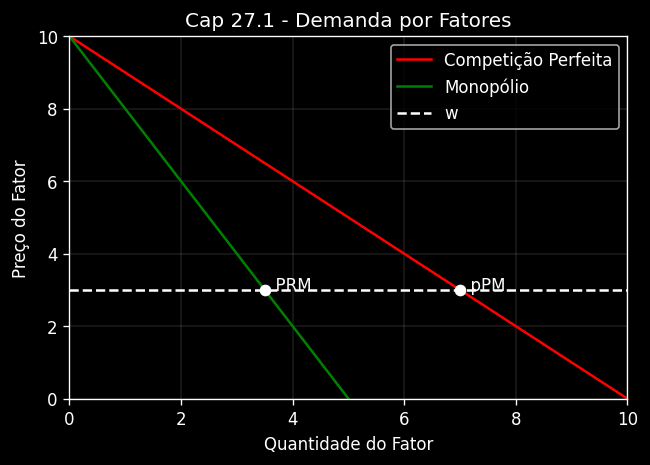
\includegraphics[scale=0.7]{cap27_1-demanda_fatores.png}
	\end{figure}

\end{frame}
%%%%%%%%%%%%%%%%%%%%%%%%%%%%%%%%%%%%%%%%%%%

\begin{frame}
	\frametitle{O Monopsônio}

	Um cenário onde temos um mercado competitivo de fatores, um único comprador de fator e um mercado de produtos competitivo.
	\\~\\
	Para simplificar, vamos supor que a empresa usa apenas um único fator de produção. Sua função de produção será dada por $y = f(x)$.  
	\\~\\
	A análise de comportamento do monopsônio é parecida com a do monopólio, só que ao invés de impactar o mercado pela oferta de bens, o poder de mercado é exercido pela compra. 
	\\~\\
	A quantidade de fator comprado, impactará no preço pago por ele.

\end{frame}

\begin{frame}
	\frametitle{O Monopsônio}

	Para expandir o modelo, vamos criar uma função de oferta inversa $w(x)$ onde o preço pago pelo insumo será determinado pela quantidade demandada pelo nosso único comprador (chamado de \textbf{monopsonista}). É razoável supor que $\frac{d w(x)}{d x} > 0$.
	\\~\\
	Num mercado de fatores competitivo, a curva de oferta de fatores é plana. Ou seja, não importando a quantidade demanda, o custo será sempre o mesmo. 
	\\~\\
	Já no caso de um único comprador, a curva de oferta de fatores será inclinada positivamente.
	\\~\\
	"Uma empresa num mercado de fatores competitivo é uma \textbf{tomadora de preços}. Um monopsionista é um \textbf{fixador de preços}".

\end{frame}

\begin{frame}
	\frametitle{O Monopsônio}

	A maximização de lucro do monoposionista será:

	\begin{center}
	\LARGE $\stackrel{max}{\text{\small $x$}} \ \ 
	\stackrel{pf(x) - w(x)x}{\ }$ \\
	\end{center}

	Ou seja, temos que encontrar a quantidade de insumo - $x$ - que permita maximizar a diferença entre a receita total - $p f(x)$ - e o custo total - $w(x)x$. A condição de primeira ordem desse problema será:

	$$ pf'(x) - [ w(x) + w'(x)x ] = 0 $$
	$$ pf'(x) = w(x) + w'(x)x $$
	$$ \underbrace{pPM_x}_{\textrm{PRM}} = \ \underbrace{w(x) + w'(x)x}_{\textrm{Custo Marginal}} $$

\end{frame}

\begin{frame}
	\frametitle{O Monopsônio}

	Como supomos no início do nosso caso, o mercado do produto é competitivo. Isso quer dizer que a receita marginal será igual a $pPM_x$ (que é a mesma coisa que $pf'(x)$). Mas obter o custo marginal não será tão simples quanto antes.
	\\~\\
	Quando a firma compra uma pequena quantidade ($x$) do fator de produção, ela deve pagar o preço desse fator vezes a quantidade ($wx$). Contudo, nesse caso, o preço será afetado exatamente na quantidade demanda ($w'(x)x$). O valor final pago é a soma dessas duas ações.
	\\~\\
	Podemos desenvolver essa lógica exatamente como desenvolvemos a receita do monopolista na seção 25.1.

\end{frame}

\begin{frame}
	\frametitle{O Monopsônio}

	$$ \Delta c = w \Delta x + x \Delta w $$
	$$ \frac{\Delta c}{\Delta x} = w + x \frac{\Delta w}{\Delta x} $$
	$$ = w \left[ 1 + \frac{x}{w} \frac{\Delta w}{\Delta x} \right] $$
	$$ = w \left[1 + \frac{1}{\eta} \right] $$

	Onde $\eta$ representa a elasticidade da oferta. Como a inclinação a curva de oferta é positiva, $\eta$ será maior que zero. 
	\\~\\
	Se a elasticidade da oferta for perfeita, $eta$ será infinito. O que implica, por sua vez, no caso da competição perfeita onde o custo marginal seria igual a $w$.

\end{frame}

\begin{frame}
	\frametitle{O Monopsônio}

	\begin{figure}[H]
		\centering
		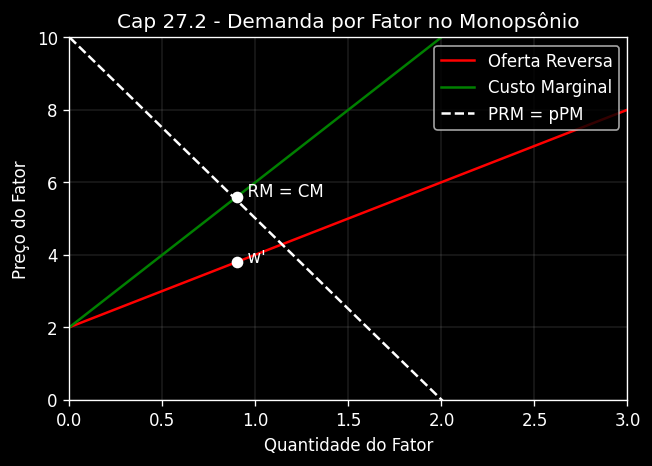
\includegraphics[scale=0.7]{cap27_2-demanda_fatores_monopsonio.png}
	\end{figure}

\end{frame}
%%%%%%%%%%%%%%%%%%%%%%%%%%%%%%%%%%%%%%%%%%%

\begin{frame}
	\frametitle{Monopólios Upstream e Downstream na Cadeia de Produção}

	Nós só observamos dois tipos de concorrência imperfeita. Mas os exemplos acima são apenas um dos múltiplos arranjos que podem acontecer na realidade.
	\\~\\
	O importante é saber como modelar o comportamento do monopolista (ou do monopsionista) seja no mercado de fatores ou no mercado de produção.
	\\~\\
	Ainda veremos uma nova situação: O caso onde um monopolista no mercado de fatores vende para um monopolista no mercado de produção.

\end{frame}

\begin{frame}
	\frametitle{Monopólios Upstream e Downstream na Cadeia de Produção}

	O monopolista do mercado de fatores é chamado de \textbf{upstream} ou \textbf{para trás}. Ele vende o insumo $x$ ao preço $k$ e com custo marginal constante $c$. 
	\\~\\
	O monopolista do mercado de produto será denominado por \textbf{downstream} ou \textbf{para frente}. Esse segundo usará o insumo $x$ para obter a produção  $y$ via função de produção da forma $f(x) = y$ que será vendida no mercado cuja demanda inversa será $p(y)$. 
	\\~\\
	No nosso exemplo a forma funcional dessa demanda será $p(y) = a - by$.

\end{frame}

\begin{frame}
	\frametitle{Monopólios Upstream e Downstream na Cadeia de Produção}

	Vamos supor que $f(x) = y = x$, ou seja, é como se ele revendesse o produto\footnote{O que torna esse exemplo surpreendentemente válido para diversas ocasiões da vida real.}. 
	\\~\\
	Outra simplificação é que o downstream também terá custo marginal igual ao preço pago pelo insumo ($k$) ao upstream.
	\\~\\
	Teremos que buscar um equilíbrio entre os dois monopolistas. Para isso, vamos começar modelando o caso para o downstream. 

\end{frame}

\begin{frame}
	\frametitle{Monopólios Upstream e Downstream na Cadeia de Produção}

	Ele quer maximizar seu lucro que é dado pelo seguinte problema:

	\begin{center}
		\Large $\stackrel{max}{\text{\small $y$}} \ \ \stackrel{L(y)\ =\ p(y)y - ky}{\ }$ \\
		\end{center}
		\begin{center}
		\Large $\stackrel{max}{\text{\small $y$}} \ \ \stackrel{L(y)\ =\ [a - by]y - ky}{\ }$ \\
		\end{center}
		\begin{center}
		\Large $\stackrel{max}{\text{\small $y$}} \ \ \stackrel{L(y)\ =\ ay - by^2 - ky}{\ }$ \\
	\end{center}

	A condição de primeira ordem da última forma é dada por:

	$$ \frac{d L(y)}{d y} = a - 2by - k = 0 $$
	$$ a - 2by = k $$
	$$ y = \frac{a - k}{2b} $$

\end{frame}

\begin{frame}
	\frametitle{Monopólios Upstream e Downstream na Cadeia de Produção}

	Como a função de produção usada iguala a quantidade de insumo à quantidade de produto. Vemos que ele demandará exatamente a mesma quantidade de fator de produção que a oferta no mercado do produto.

	$$ y = x = \frac{a - k}{2b} $$

	O importante aqui é perceber que a função de produção do monopolista downstream é usada para derivar a demanda do fator produzido pelo upstream. 
	\\~\\
	Perceba que a quantidade demandada de fator depende do preço pago por ele e da demanda no mercado de produto. Tudo bem intuitivo e simples.

\end{frame}

\begin{frame}
	\frametitle{Monopólios Upstream e Downstream na Cadeia de Produção}

	Agora temos que modelar o comportamento do upstream. Vamos supor que ele tenha acesso à função demanda de fatores do downstream e queira maximizar seu lucro.

	A demanda inversa de fatores nada mais é do que a última equação tendo k em função de x:

	$$ k(x) = a - 2bx $$

	A receita é dada por:

	$$ k(x)x = ax - 2bx^2 $$

	E a receita marginal por:

	$$ RM_x = a - 4bx $$

\end{frame}

\begin{frame}
	\frametitle{Monopólios Upstream e Downstream na Cadeia de Produção}

	Igualando a receita marginal ao custo marginal, teremos que:

	$$ a - 4bx = c $$

	ou seja, o total vendido no mercado pelo monopolista upstream será dado por:

	$$ x = \frac{a - c}{4b} $$

	Como a função de produção é um pra um, podemos definir que o total produzido no mercado de produto será:

	$$ y = \frac{a - c}{4b} $$

	Essa é a quantidade da produção que maximiza os lucros do monopolista upstream.

\end{frame}

\begin{frame}
	\frametitle{Monopólios Upstream e Downstream na Cadeia de Produção}

	Lembre-se que ele usa como função de demanda de fatores o resultado do problema de maximização do downstream. Então a solução acaba por gerar um lucro fruto do processo de maximização de ambos os monopolistas.
	\\~\\
	Se houvesse apenas um monopolista em ambos os mercados (imagine que as duas empresas se fundissem) e os custos de produção dos fatores se mantivessem os mesmos.
	\\~\\
	O problema de maximização seria igualar a receita marginal ($a - 2by$) ao custo do fator ($c$). Isso geraria um volume de produção igual à

	$$ y_{int} = \frac{a - c}{2b}$$

\end{frame}

\begin{frame}
	\frametitle{Monopólios Upstream e Downstream na Cadeia de Produção}

	O monopolista integrado produzirá o dobro que o arranjo com dois monopolistas separados. Mas qual o motivo dessa diferença?
	\\~\\
	Na prática, o monopolista upstream vai cobrar uma quantidade cujo preço de mercado é superior ao custo marginal. 
	\\~\\
	Esse preço será o custo que o monopolista downstream usará para maximizar seu lucro. 
	\\~\\
	Contudo, quando as empresas se fundem, o novo custo marginal do monopolista do mercado de produto será exatamente o custo de produção $c$. Nós retiramos de cena o Markup do monopolista upstream.

\end{frame}

%%%%%%%%%%%%%%%%%%%%%%%%%%%%%%%%%%%%%%%%%%%
\section{Oligopólio}
%%%%%%%%%%%%%%%%%%%%%%%%%%%%%%%%%%%%%%%%%%%

\begin{frame}
	\huge O Oligopólio \normalsize
	\\~\\
	\begin{itemize}
		\item A Escolha de uma Estratégia
		\item Liderança na Quantidade
		\item Liderança no Preços
		\item Estabelecimento Simultâneo da quantidade (Equilíbrio de Cournot)
		\item Ajustamento para o Equilíbrio
		\item Várias Empresas no Equilíbrio de Cournot
		\item Fixação Simultânea de Preços
		\item Conluio
		\item Estratégias Punitivas
		\item Comparação das Soluções
	\end{itemize}
\end{frame}

\begin{frame}
	\frametitle{O Oligopólio}

	Pensemos em uma situação onde temos poucos concorrentes.
	\\~\\
	De um lado, não temos tantos a ponto de ninguém poder manipular seus preços.
	\\~\\
	Do outro, ninguém é grande o suficiente para ignorar o comportamento dos seus concorrentes. 
	\\~\\
	Esse arranjo é denominado de \textbf{Oligopólio}.
	\\~\\
	Vamos partir da estrutura de competição de apenas duas empresas: o \textbf{Duopólio}. Outra limitação que imporemos é a de que os produtos são idênticos.
	\\~\\
	Nosso foco são as \textbf{interações estratégicas}.

\end{frame}

\begin{frame}
	\frametitle{A Escolha de uma Estratégia}

	Em um arranjo de dois competidores, temos que desenvolver um modelo que consiga equilibrar 4 variáveis:

	\begin{itemize}
		\item Preço da Empresa 1
		\item Preço da Empresa 2
		\item Quantidade da Empresa 1
		\item Quantidade da Empresa 2
	\end{itemize}
	\ 
	\\~\\
	Quando as duas empresas decidem sem ter acesso a informação do adversário, elas precisam supor o que ele fará. Esse arranjo é denominado \textbf{jogo simultâneo}.

\end{frame}

\begin{frame}
	\frametitle{A Escolha de uma Estratégia}

	Chamaremos de \textbf{líder} toda empresa que decidir seu \textbf{preço} ou \textbf{quantidade} antes da outra. 
	\\~\\
	A empresa que decidirá após a informação da decisão da empresa líder será chamada de \textbf{seguidora}. 
	\\~\\
	As interações desse tipo são chamadas de \textbf{jogos sequenciais}.

\end{frame}


\begin{frame}
	\frametitle{A Escolha de uma Estratégia}

	Com esses dois conceitos, podemos ter 4 tipos de interações estratégicas:

	\begin{itemize}
		\item Liderança de Preço
		\item Liderança de Quantidade
		\item Preço Simultâneo
		\item Quantidade Simultânea
	\end{itemize}
	\ 
	\\~\\
	Além dessas, veremos uma opção possível de estratégia onde há negociação entre as empresas para formação de um \textbf{conluio}. Esse tipo de esquema é chamado de \textbf{jogo cooperativo}.

\end{frame}

\begin{frame}
	\frametitle{Liderança na Quantidade}

	O modelo desenvolvido nessa seção é creditado ao economista alemão Heinrich von Stackelberg. Seu livro \textit{Marktform und Gleichgewicht} foi publicado em 1934.
	\\~\\
	Vamos supor que temos uma empresa líder na quantidade. Ela fixará sua produção em $y_1$ unidades.
	\\~\\
	A empresa seguidora, de posse da informação de $y_1$ e da demanda inversa do mercado, escolherá seu nível de produção em $y_2$.
	\\~\\
	A demanda inversa do mercado será em função do total de produtos $p(Y) = p(y_1 + y_2)$.

\end{frame}

\begin{frame}
	\frametitle{Liderança na Quantidade}

	Como a empresa líder decidirá sua quantidade de modo a maximizar seus lucros?
	\\~\\
	Não seria nada estranho que ela tivesse a hipótese que a empresa seguidora queira maximizar seus lucros também.
	\\~\\
	Desse modo, a empresa líder terá que endogenizar o problema da maximização do lucro da empresa seguidora.
	\\~\\
	O problema da maximização da empresa seguidora é:

	\begin{center}
	\LARGE $\stackrel{max}{\text{\small $y_2$}} \ \ \stackrel{p(y_1 + y_2)y_2 - c_2(y_2)}{\ }$ \\
	\end{center}

\end{frame}

\begin{frame}
	\frametitle{Liderança na Quantidade}

	Queremos encontrar o ponto onde a receita marginal será igual ao custo marginal.

	$$ RM_2 = CMa_2 = p(y_1 + y_2) + \frac{dp(y_1+y_2)}{dy_2}y_2 - \frac{dc_2(y_2)}{y_2} = 0 $$

	A novidade aqui é que temos que levar em consideração a quantidade $y_1$ para encontrar nosso $y_2$. Isso quer dizer que 

	$$y_2 = f_2(y_1)$$

\end{frame}

\begin{frame}
	\frametitle{Liderança na Quantidade}

	Nós conseguimos obter essa função isolando nosso termo $y_2$ no problema de maximização acima.
	\\~\\
	Essa função tem o nome de \textbf{função de reação} e nos diz qual quantidade será produzida pela empresa seguidora ao ser conhecida a quantidade da empresa líder.
	\\~\\
	Vamos definir a função de demanda inversa como $p(y_1 + y_2) = a - b(y_1 + y_2)$ e também adotaremos o custo igual a zero para facilitar a matemática da coisa.

\end{frame}

\begin{frame}
	\frametitle{Liderança na Quantidade}

	$$\textrm{Função Lucro 2: } \pi_2(y_1,y_2) = p(y_1 + y_2)y_2$$
	
	$$ = [a - b(y_1 + y_2)]y_2 = ay_2 - by_1 y_2 - by_2^2 $$

	Com a função de lucro e a de reação, conseguimos ver a relação entre essas duas funções. 
	\\~\\
	Na imagem abaixo podemos ver que a curva de reação sempre atravessa as curvas de isolucro no ponto onde temos o maior valor de $y_2$.

\end{frame}

\begin{frame}
	\frametitle{Liderança na Quantidade}

	\begin{figure}[H]
		\centering
		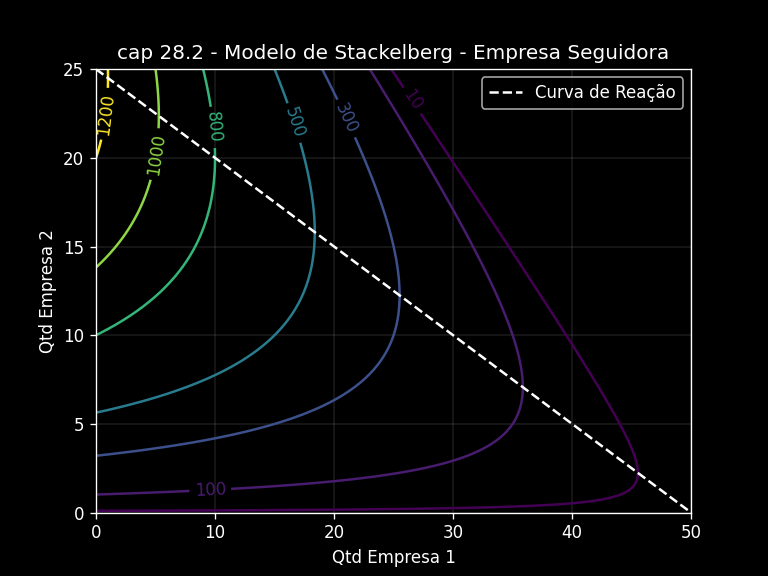
\includegraphics[scale=0.55]{cap28_2-modelo_stackelberg_parcial.png}
	\end{figure}
	
\end{frame}

\begin{frame}
	\frametitle{Liderança na Quantidade}

	Agora vamos desenvolver como essa empresa define a sua quantidade de modo a maximizar o seu lucro.
	\\~\\
	Uma das características desse modelo é que a empresa líder conhece $f_2(y_1)$.

	\begin{center}
		\LARGE $\stackrel{max}{\text{\small $y_1$}} \ \ \stackrel{p(y_1 + y_2)y_1 - c_1(y_1)}{\ }$ \\
		\small de modo que \normalsize $y_2 = f_2(y_1)$
	\end{center}

	Ou melhor

	\begin{center}
		\LARGE $\stackrel{max}{\text{\small $y_1$}} \ \ \stackrel{p[y_1 + f_2(y_1)]y_1 - c_1(y_1)}{\ }$ \\
	\end{center}
		
\end{frame}

\begin{frame}
	\frametitle{Liderança na Quantidade}

	A produção total será definida pela líder sendo que será parte devida a produção direta e a outra parte pela resposta da seguidora ao nível definido da produção, ou seja, $y_1 + f_2(y_1)$.
	\\~\\
	Pela equação da demanda inversa linear, temos que a função de reação da empresa seguidora é

	$$ f_2(y_1) = y_2 = \frac{a - by_1}{2b}$$

	A função lucro é dada pela receita menos os custos (que no nosso exemplo é zero)

	$$ \textrm{Função Lucro 1: } \pi(y_1,y_2) = [a - b(y_1 + y_2)]y_1 = ay_1 -by_1^2 - by_1y_2 $$

\end{frame}

\begin{frame}
	\frametitle{Liderança na Quantidade}

	Colocando a função de reação dentro da função de lucro teremos

	$$ = ay_1 -by_1^2 - by_1f(y_1)$$
	$$ = ay_1 -by_1^2 - by_1\frac{a - by_1}{2b}$$
	$$ = ay_1 -by_1^2 - \frac{\cancel{b}y_1a}{2\cancel{b}} + \frac{\cancel{b}*b(y_1)^2}{2\cancel{b}}$$
	$$= ay_1 -by_1^2 - \frac{ay_1}{2} + \frac{by_1^2}{2}$$
	$$ \pi(y_1,y_2) = \frac{a}{2}y_1 - \frac{b}{2}y_1^2$$

\end{frame}

\begin{frame}
	\frametitle{Liderança na Quantidade}

	Para encontrarmos a quantidade ótima basta derivar a função lucro em função de $y_1$ e igualar a zero. O que nos dará 

	$$ y_1^* = \frac{a}{2b} $$

	Desse modo, podemos encontrar facilmente a produção de equilíbrio da empresa seguidora.

	$$ y_2^* = \frac{a - by_1}{2b} $$
	$$ y_2^* = \frac{a - b(a/2b)}{2b} $$
	$$ y_2^* = \frac{a}{4b} $$

\end{frame}

\begin{frame}
	\frametitle{Liderança na Quantidade}

	Por fim, podemos ter a quantidade total do mercado pela soma de $y_1^* + y_2^* = \frac{3a}{4b}$. 
	\\~\\
	O ponto de Equilíbrio de Stackelberg acontecerá onde \textbf{a curva de reação tangencia a maior curva de isolucro} da empresa líder. 
	\\~\\
	No exemplo da imagem eu usei para a função da demanda inversa linear um $a = 100$ e um $b = 2$.
	\\~\\
	Agora que temos a função de lucro da empresa 1, podemos acrescentar as curvas de isolucro para vermos a solução gráfica da álgebra que acabamos de desenvolver.

\end{frame}

\begin{frame}
	\frametitle{Liderança na Quantidade}

	\begin{figure}[H]
		\centering
		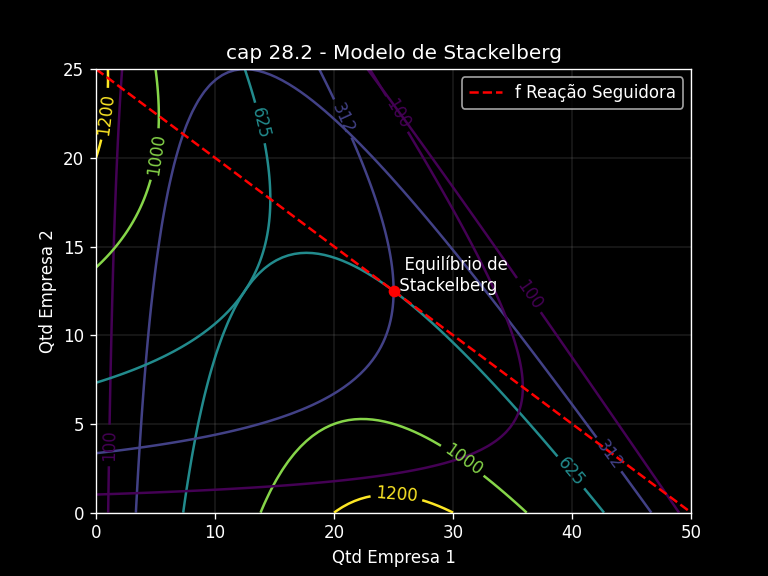
\includegraphics[scale=0.55]{cap28_2-modelo_stackelberg_completo.png}
	\end{figure}

\end{frame}

\begin{frame}
	\frametitle{Liderança no Preços}

	Outra forma de um jogo sequencial acontecer entre duas empresas é pela definição do preço pela empresa líder. 
	\\~\\
	Similarmente ao que vimos na seção anterior, a empresa líder precisa levar em consideração o que a empresa seguidora fará.
	\\~\\
	A seguidora recebe o preço definido pela líder e maximiza seu lucro.

	\begin{center}
		\LARGE $\stackrel{max}{\text{\small $y_2$}} \ \ \stackrel{py_2 - c_2(y_2)}{\ }$ \\
	\end{center}

\end{frame}

\begin{frame}
	\frametitle{Liderança no Preços}

	A empresa líder, sabendo a função de oferta da empresa seguidora, vai trabalhar com a diferença entre a Demanda do mercado e a demanda da empresa seguidora, ou seja, $R(p) = D(p) - S(p)$. 
	\\~\\
	O nome dessa curva de demanda reduzida é \textbf{curva de demanda residual}.
	\\~\\
	Supondo um custo de produção constante $c$. A função de lucro da empresa líder é dada por

	$$ \textrm{Função Lucro 1: } \pi_1(p) = R(p)p - R(p)c = (p - c)R(p) $$

\end{frame}

\begin{frame}
	\frametitle{Liderança no Preços}

	A maximização dessa empresa acontece onde a receita marginal (que nesse caso é oriunda da demanda residual) é igual ao custo marginal.
	\\~\\
	Definindo nossa demanda como $D(p) = a - bp$ e as funções custo para a seguidora $c_2(y_2) = y_2^2/2$ e para a líder $c_1(y_1) = cy_1$.
	\\~\\
	Isso nos diz que a condição de maximização da empresa seguidora será a derivada da função lucro igual a zero.

	$$ \frac{d L(y_2)}{y_2} = p - \frac{2y_2}{2} = 0 $$
	$$ = p - y_2 = 0 $$
	$$ = p = y_2 $$

\end{frame}

\begin{frame}
	\frametitle{Liderança no Preços}

	Nossa função de oferta da seguidora será $S(p) = p$. 
	\\~\\
	De posse dessa informação, podemos descobrir a equação da demanda residual da empresa líder pela subtração da curva de demanda pela oferta da seguidora.

	$$ R(p) = D(p) - S(p) = a - bp - p = a - (b + 1)p $$

	Agora é só maximizar o lucro pela igualdade entre a receita marginal e o custo marginal e verificar na curva de demanda inversa o volume de produção e o preço.

\end{frame}

\begin{frame}
	\frametitle{Liderança no Preços}

	Demanda inversa é obtida isolando $p$ da demanda residual.

	$$ p(y_1) = \frac{a}{b+1}-\frac{1}{b+1}y_1 $$

	A receita da empresa líder é obtida pela multiplicação de $p(y_1)$ por $y_1$. A receita marginal é a derivada dessa função em relação a $y_1$.

	$$ Receita_1: \left[ \frac{a}{b+1} - \frac{1}{b+1}y_1 \right] y_1 $$
	$$ = \frac{a}{b+1}y_1 - \frac{1}{b+1}y_1^2 $$

	A receita marginal será

	$$ RMa_1 = \frac{a}{b+1} - \frac{2}{b+1}y_1 $$

\end{frame}

\begin{frame}
	\frametitle{Liderança no Preços}

	O nosso custo foi definido como $c_1(y_1) = cy_1$, logo, o custo marginal é igual a $c$.
	\\~\\
	Portanto, nosso problema de maximização será dado pela equação

	$$ \frac{a}{b+1} - \frac{2}{b+1}y_1 = c $$
	$$ y_1^* = \frac{c(b+1)}{2} $$

	Na imagem, nós podemos ver as variáveis interagindo. A oferta total será a soma das quantidades de ambas empresas. Por acaso, a oferta da seguidora está igual à receita marginal da líder mas isso é só um acaso.

\end{frame}

\begin{frame}
	\frametitle{Liderança no Preços}

	\begin{figure}[H]
		\centering
		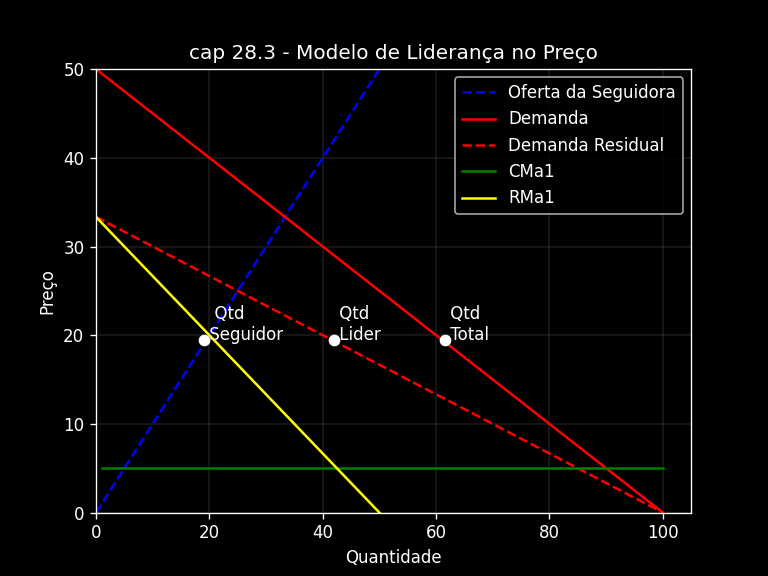
\includegraphics[scale=0.55]{cap28_3-lideranca_preco.png}
	\end{figure}

\end{frame}

\begin{frame}
	\frametitle{Estabelecimento Simultâneo da quantidade}

	Não é comum que as empresas fiquem se comunicando para informar seus concorrentes a respeito de suas decisões.
	\\~\\
	Nesses cenários, as empresas precisam supor o que suas concorrentes farão.
	\\~\\
	Esse modelo é chamado de \textbf{Modelo de Cournot} e é um modelo de jogo simultâneo onde as empresas definem suas quantidades produzidas e vendidas no mercado.
	\\~\\
	Suporemos que as empresas queiram maximizar seus lucros.

\end{frame}

\begin{frame}
	\frametitle{Estabelecimento Simultâneo da quantidade}

	A quantidade total do mercado será dada por $Y = y_1 + y_2^e$, onde $y_2^e$ é a quantidade prevista da empresa 2. 
	\\~\\
	O preço de equilíbrio do mercado será dado pela equação de demanda inversa $p(Y) = p(y_1 + y_2^e)$.
	\\~\\
	O problema de maximização do lucro será

	\begin{center}
		\LARGE $\stackrel{max}{\text{\small $y_1$}} \ \ \stackrel{p(y_1 + y_2^e)y_1 - c(y_1)}{\ }$ \\
	\end{center}

\end{frame}

\begin{frame}
	\frametitle{Estabelecimento Simultâneo da quantidade}

	Existe uma relação entre essa expectativa e a produção, de modo mais formal, $y_1 = f(y_2^e)$.
	\\~\\
	Essa é a \textbf{curva de reação} da empresa, a diferença é que aqui a empresa 1 não é mais a líder e essa reação se refere a \textit{expectativa} da produção. Mas o tratamento matemático é o mesmo.
	\\~\\
	Similarmente, a empresa 2 se depara com a mesma situação.

	$$y_2 = f(y_1^e)$$

\end{frame}

\begin{frame}
	\frametitle{Estabelecimento Simultâneo da quantidade}

	O equilíbrio de Cournot é dado pelo sistemas de equações

	$$ y_1^* = f_1(y_2^*) $$
	$$ y_2^* = f_2(y_1^*) $$

	Nenhuma das empresas terá incentivos em mudar seu nível de produção.
	\\~\\
	Se reutilizarmos o exemplo na liderança da quantidade (com custo zero e demanda linear) obteremos as mesmas funções de reação que a empresa 2 tinha naquele modelo.

\end{frame}

\begin{frame}
	\frametitle{Estabelecimento Simultâneo da quantidade}

	$$ y_1 = \frac{a - by_2^e}{2b} $$

	e

	$$ y_2 = \frac{a - by_1^e}{2b} $$

	O ponto de equilíbrio acontece onde $y_1 = y_2$, ou seja, onde as curvas de reação são iguais. Nesse ponto, $y_1^e = y_1$ e $y_2^e = y_2$. 
	\\~\\
	Só precisamos substituir dentro desse sistema de equações do seguinte modo

\end{frame}

\begin{frame}
	\frametitle{Estabelecimento Simultâneo da quantidade}

	$$ y_1 = \frac{a - by_2^e}{2b} $$
	$$ y_1 = \frac{a - by_2}{2b} $$
	$$ y_1 = \frac{a - b(\frac{a - by_1}{2b})}{2b} $$
	$$ y_1^* = \frac{a}{3b} = y_2^* $$

	Com essas funções e as equações de lucro podemos ver graficamente o equilíbrio de Cournot onde as curvas de reação se equivalem.

\end{frame}

\begin{frame}
	\frametitle{Estabelecimento Simultâneo da quantidade}

	\begin{figure}[H]
		\centering
		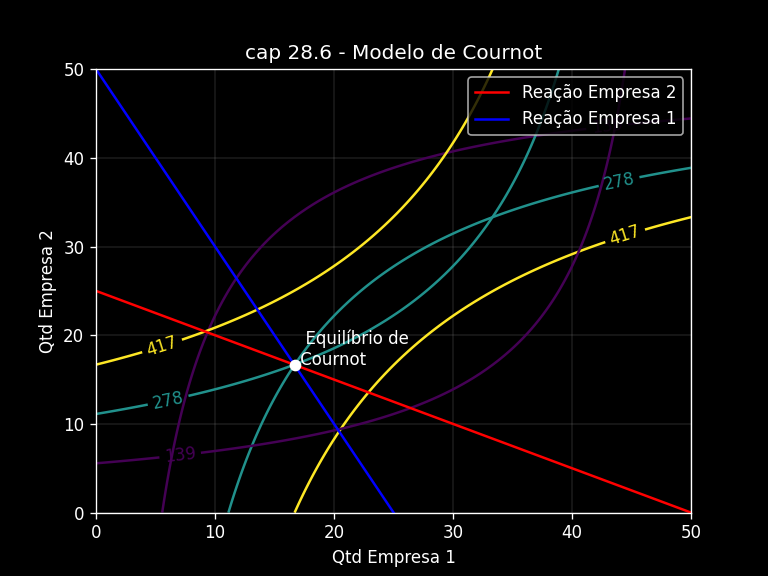
\includegraphics[scale=0.55]{cap28_6-modelo_cournot.png}
	\end{figure}
	
\end{frame}

\begin{frame}
	\frametitle{Ajustamento para o Equilíbrio}

	Seria muita boa vontade supor que, na vida real, as empresas conseguissem acertar na mosca o nível de produção dos seus concorrentes. 
	\\~\\
	Mas o nosso modelo é forte o suficiente para um processo de ajustamento em caso de (prováveis) palpites equivocados no nível de produção.
	\\~\\
	Vamos supor que a cesta inicial produzida esteja em cima da curva de reação da empresa 2. A cesta inicial, que chamamos no gráfico de $Cesta(t)$ será igual à lista $(y_1^t,y_2^t)$.
	\\~\\
	Essa cesta está na curva de reação da empresa 2, logo, essa empresa não terá incentivo a fazer nenhuma mudança. Mas para a empresa 1, a situação é outra, ela quer reduzir sua produção para aumentar seus lucros.

\end{frame}

\begin{frame}
	\frametitle{Ajustamento para o Equilíbrio}

	\begin{figure}[H]
		\centering
		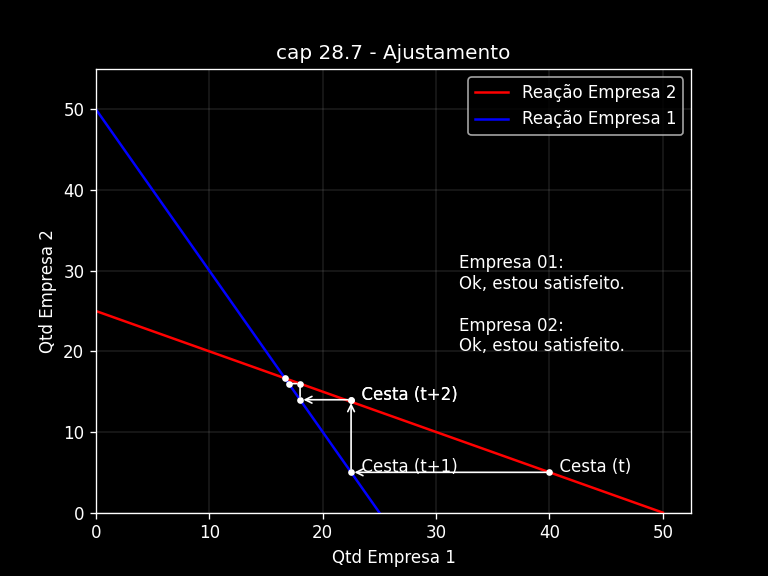
\includegraphics[scale=0.55]{cap28_7-ajustamento.png}
	\end{figure}

\end{frame}


\begin{frame}
	\frametitle{Várias Empresas no Equilíbrio de Cournot}

	A oferta total da indústria será dada por $Y = y_1 + y_2 + \dots + y_{n-1} + y_n$. Desse modo o problema da maximização da empresa será dado pela igualdade entre a receita marginal e o seu custo marginal do seguinte modo

	$$ p(Y) + \frac{\delta p}{\delta Y} y_i = CMa(y_i) $$
	$$ p(Y) + \frac{\delta p}{\delta Y} \frac{Y}{Y} \frac{p(Y)}{p(Y)} y_i = CMa(y_i) $$
	$$ p(Y) \left[1 + \frac{\delta p}{\delta Y} \frac{Y}{p(Y)} \frac{y_i}{Y} \right] = CMa(y_i) $$

\end{frame}

\begin{frame}
	\frametitle{Várias Empresas no Equilíbrio de Cournot}

	Definindo $s_i = \frac{y_i}{Y}$ como a participação da empresa no total do mercado.

	$$ p(Y) \left[1 + \frac{\delta p}{\delta Y} \frac{Y}{p(Y)} s_i \right] = CMa(y_i) $$

	Se lembrarmos da fórmula da elasticidade, podemos ver que o termo $\frac{\delta p}{\delta Y} \frac{Y}{p(y)}$ é justamente o inverso da elasticidade $\frac{1}{\epsilon(Y)}$

	$$ p(Y) \left[1 - \frac{s_i}{|\epsilon(Y)|} \right] = CMa(y_i) $$

	Que é o mesmo que

	$$ p(Y) \left[1 - 1/\frac{|\epsilon(Y)|}{s_i} \right] = CMa(y_i) $$

\end{frame}

\begin{frame}
	\frametitle{Várias Empresas no Equilíbrio de Cournot}

	Essa solução é bem parecida com a maximização do monopolista. 
	\\~\\
	A principal diferença é esse termo $s_i$ dividindo a elasticidade. 
	\\~\\
	Como $s_i = y_i/Y$ ele será $0 \leq s_i \leq 1$. 
	\\~\\
	No caso monopolista, sabemos que $s_i = 1$. No outro extremo, se $lim (s_i) \rightarrow 0$, a empresa terá elasticidade infinita como as empresas da competição perfeita.
	\\~\\
	Quanto maior $s_i$ menor será a elasticidade da demanda da empresa.
\end{frame}

\begin{frame}
	\frametitle{Fixação Simultânea de Preços}

	Em algum momento do século XIX, um matemático francês de nome Joseph Bertrand, ao ler o livro do Cournot, desenvolveu um modelo simultâneo de equilíbrio de preços. 
	\\~\\
	Esse modelo ficou conhecido como \textbf{concorrência de Bertrand}.

\end{frame}

\begin{frame}
	\frametitle{Fixação Simultânea de Preços}

	Estamos na busca do par de preços que permitam ambas as empresas maximizar seus lucros. Para isso, temos que seguir algumas regras vindas dos modelos de maximização já vistos até agora:

	\begin{itemize}
		\item O preço não poderá ser maior que o custo marginal porque as empresas aumentariam seus lucros simplesmente produzindo menos.
		\item Se o preço for maior que o custo marginal, todas as empresas terão um incentivo de reduzir seu preço para "roubar"\ os clientes das concorrentes e ainda auferir lucros positivos.
	\end{itemize}
	
\end{frame}

\begin{frame}
	\frametitle{Fixação Simultânea de Preços}

	O segundo ponto funciona de maneira recursiva. 
	\\~\\
	Se uma empresa reduz seu preço em $10\%$ abaixo dos preços das suas concorrentes, ela ganhará parte do mercado. 
	\\~\\
	As concorrentes terão o incentivo em reduzir mais ainda seus preços até o ponto onde não poderão mais reduzir (determinado pelo custo marginal).
	\\~\\
	O ponto onde não será possível reduzir os preços é justamento a igualdade do custo marginal. Que é a imposição 1 do nosso modelo. Esse é precisamente o equilíbrio de Bertrand.

\end{frame}

\begin{frame}
	\frametitle{Conluio}

	

\end{frame}

\begin{frame}
	\frametitle{Estratégias Punitivas}

	

\end{frame}

\begin{frame}
	\frametitle{Comparação das Soluções}

	

\end{frame}


%%%%%%%%%%%%%%%%%%%%%%%%%%%%%%%%%%%%%%%%%%%

\begin{frame}
	\frametitle{}

	

\end{frame}

\end{document}

